%!TEX root = free234.tex
%!TEX program=xelatex
% Time-stamp: <2015-10-23 17:44:27 angenent>
\chapter{Maxima and Minima}  
In first semester calculus we learned how to find the maximal and minimal values of a
function $y=f(x)$ of one variable.  The basic method is as follows: assuming the
independent variable is restricted to some interval $a\leq x\leq b$, we first look
for interior maxima and minima.  These always occur at \emph{critical} or
\emph{stationary} points of the function, i.e.\ solutions $x$ of $f'(x)=0$.  We then
check the function values at the endpoints $a$ and $b$ of the interval, to see if
they might be maxima or minima.

To find out which solutions of $f'(x)=0$ are actually local maxima or minima we can look
at the sign of the derivative $f'(x)$ to see where the function is increasing or
decreasing, or we can apply the \emph{second derivative test.}

This chapter we will see how to solve similar questions about functions of two
or more variables.

\section{Local and Global extrema}     

\label{sec:local-versus-global} 
Let $z=f(x,y)$ be the function whose maximal or minimal values we are looking
for, and let $D$ be the domain of this function.  This domain could be the
largest possible domain for the given function (in case $f$ is defined by a
formula), but it could also be some smaller region which we ourselves have
chosen.  The question we are considering is
\begin{center}
  \itshape What are the largest and smallest values that $f(x,y)$ can have\\
  if the point $(x,y)$ belongs to the domain $D$?
\end{center}
\subsection{Definition of global extrema}     

\label{sec:def-global-extrema}\itshape 
The function $f$ has a \emph{global maximum} or \emph{absolute maximum} at a
point $(a,b)$ in $D$ if $f(x,y)\leq f(a,b)$ for all points $(x,y)$ in $D$.

\upshape%
Similarly,\itshape\ the function $f$ has a \emph{global minimum} or
\emph{absolute minimum} at a point $(a,b)$ in $D$ if $f(x,y)\geq f(a,b)$ for all
points $(x,y)$ in $D$.

\subsection{Definition of local extrema}     

\label{sec:def-local-extrema}\itshape 
The function $f$ has a \emph{local maximum} at a point $(a,b)$ in $D$ if there
is a $r>0$ such that $f(x,y)\leq f(a,b)$ for all points $(x,y)$ in $D$ which
also lie in a disc of radius $r$ centered at $(a,b)$.  \upshape

Local minima are defined analogously.

\subsection{Interior extrema}     

\label{sec:interior-extrema} 
Recall that a point $(a,b)$ in a domain $D$ is called \emph{interior} if it is
not a boundary point, or, more precisely, if there is some small $r>0$ such that
the disc with radius $r$ centered at $(a,b)$ is entirely contained in $D$.  We
will apply this distinction to the local and global maxima and minima that we
find: an \emph{interior local minimum} is a local minimum that occurs at an
interior point of the domain $D$ of the function.


\section{Continuous functions on closed and bounded sets}     
Before we go into the details of how we can actually find the maxima and minima,
it is good to know the following general fact. It tells us where to expect
maxima and minima.

Let $z=f(x_1,\ldots,x_n)$ be a continuous function defined on some \emph{closed} and
\emph{bounded} region $D$ in $\R^n$.  Here ``closed'' means that $D$ contains all its
boundary points, and ``bounded'' means that all points in $D$ are no further away
from the origin than some fixed radius $R$ ($D$ does not ``stretch all the way to
infinity''.)

We will also assume that $f$ is continuous on $D$.

\subsection{Theorem about Maxima and Minima of Continuous Functions}     
\label{thm:maxmin-exist}%
\itshape%
A continuous function defined on a closed and bounded region $D\subset \R^n$ has
both a maximum and minimum within that region.  \upshape

The precise definitions of the concepts (continuous, closed, bounded) and the
proof of this theorem all involve a fair number of $\varepsilon$'s and
$\delta$'s.  This material is treated in courses like Math 421, 521 (real
analysis) or 551 (point set topology) and really does not belong here in Math
234.  Nevertheless it is important to have some understanding of what is meant
in the above theorem.  The following examples are meant to clarify this.


\subsection{Example -- The function $f(x, y) = x^2+y^2$}

\label{sec:examples-maxmin-existence}
\begin{figure}[tb]
  \centering
  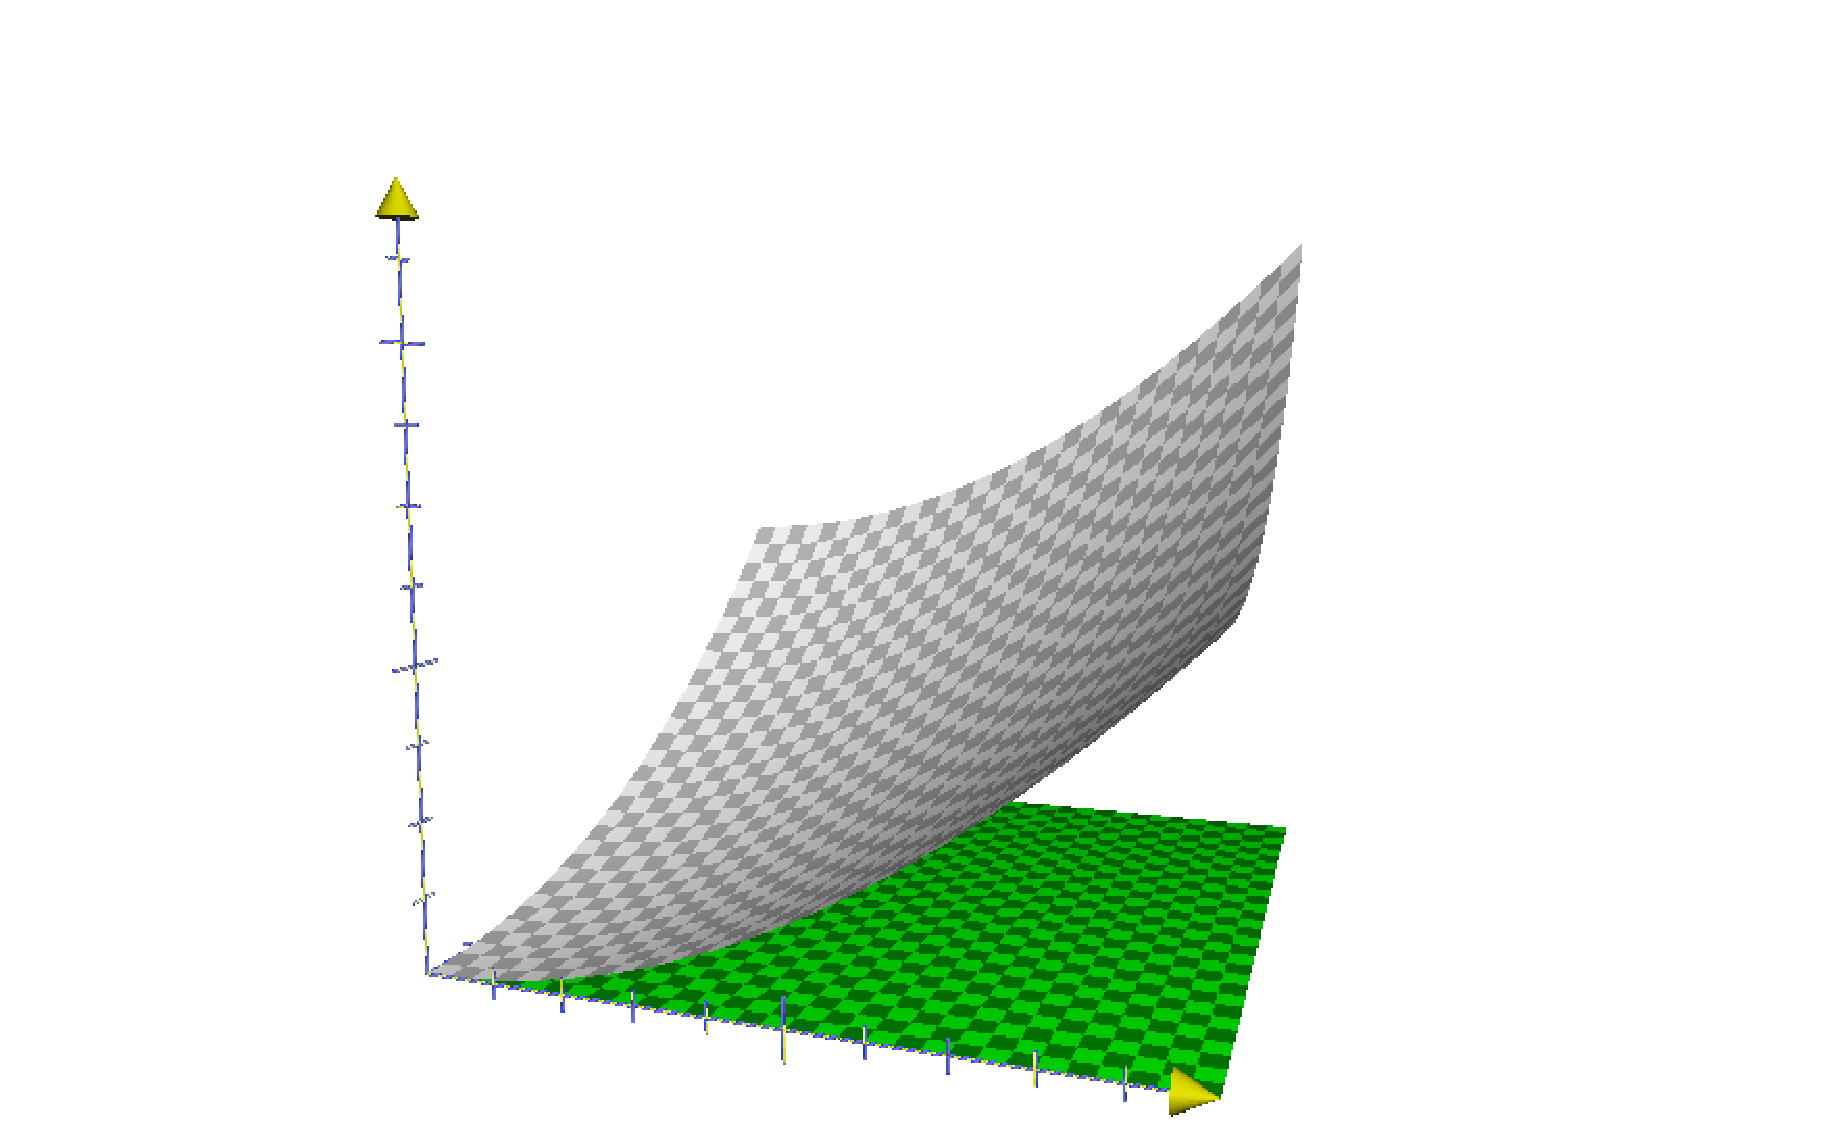
\includegraphics[width=100pt]{03maxmin-on-square.pdf}
  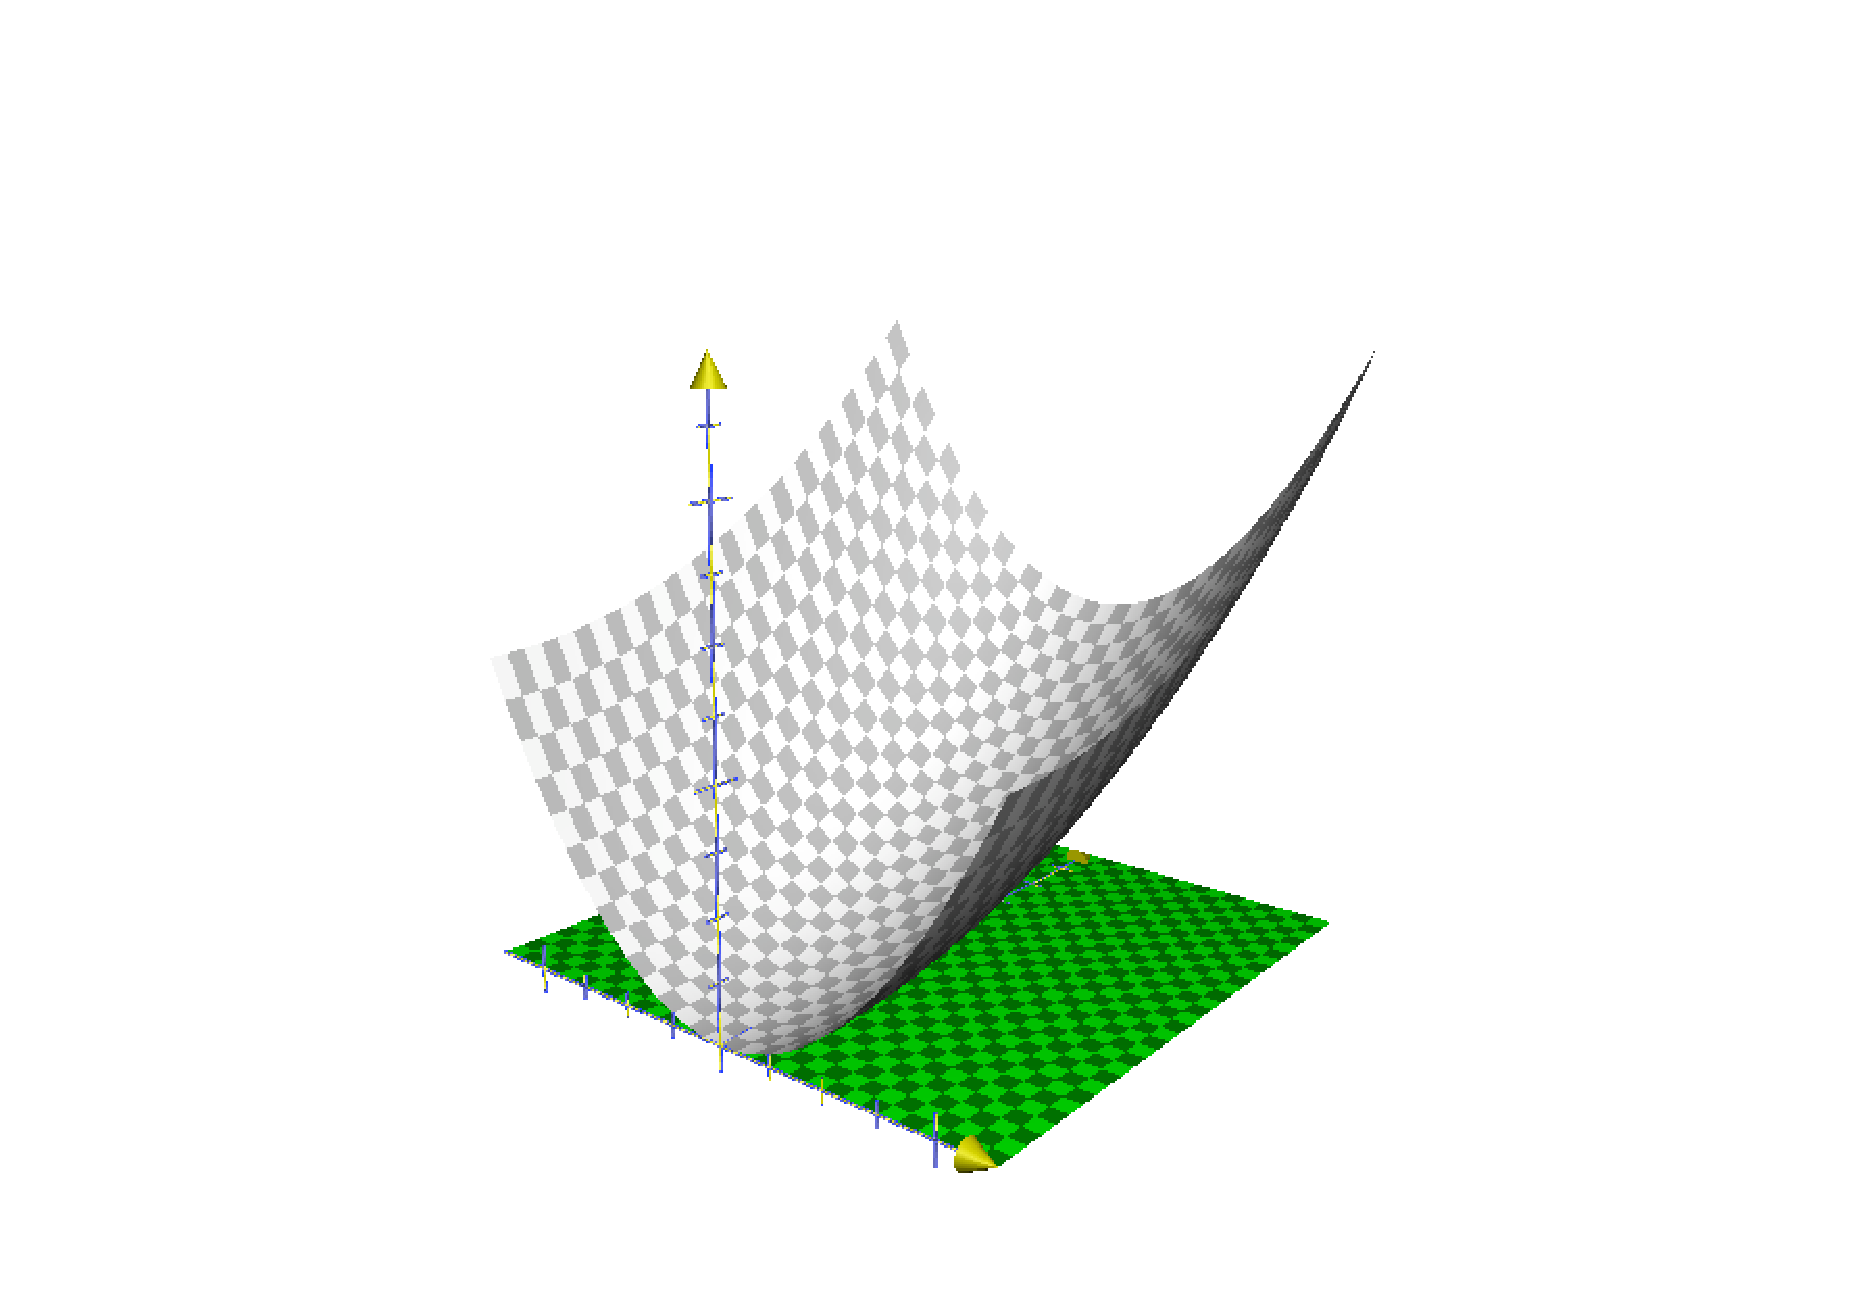
\includegraphics[width=100pt]{03maxmin-on-square2.pdf}
  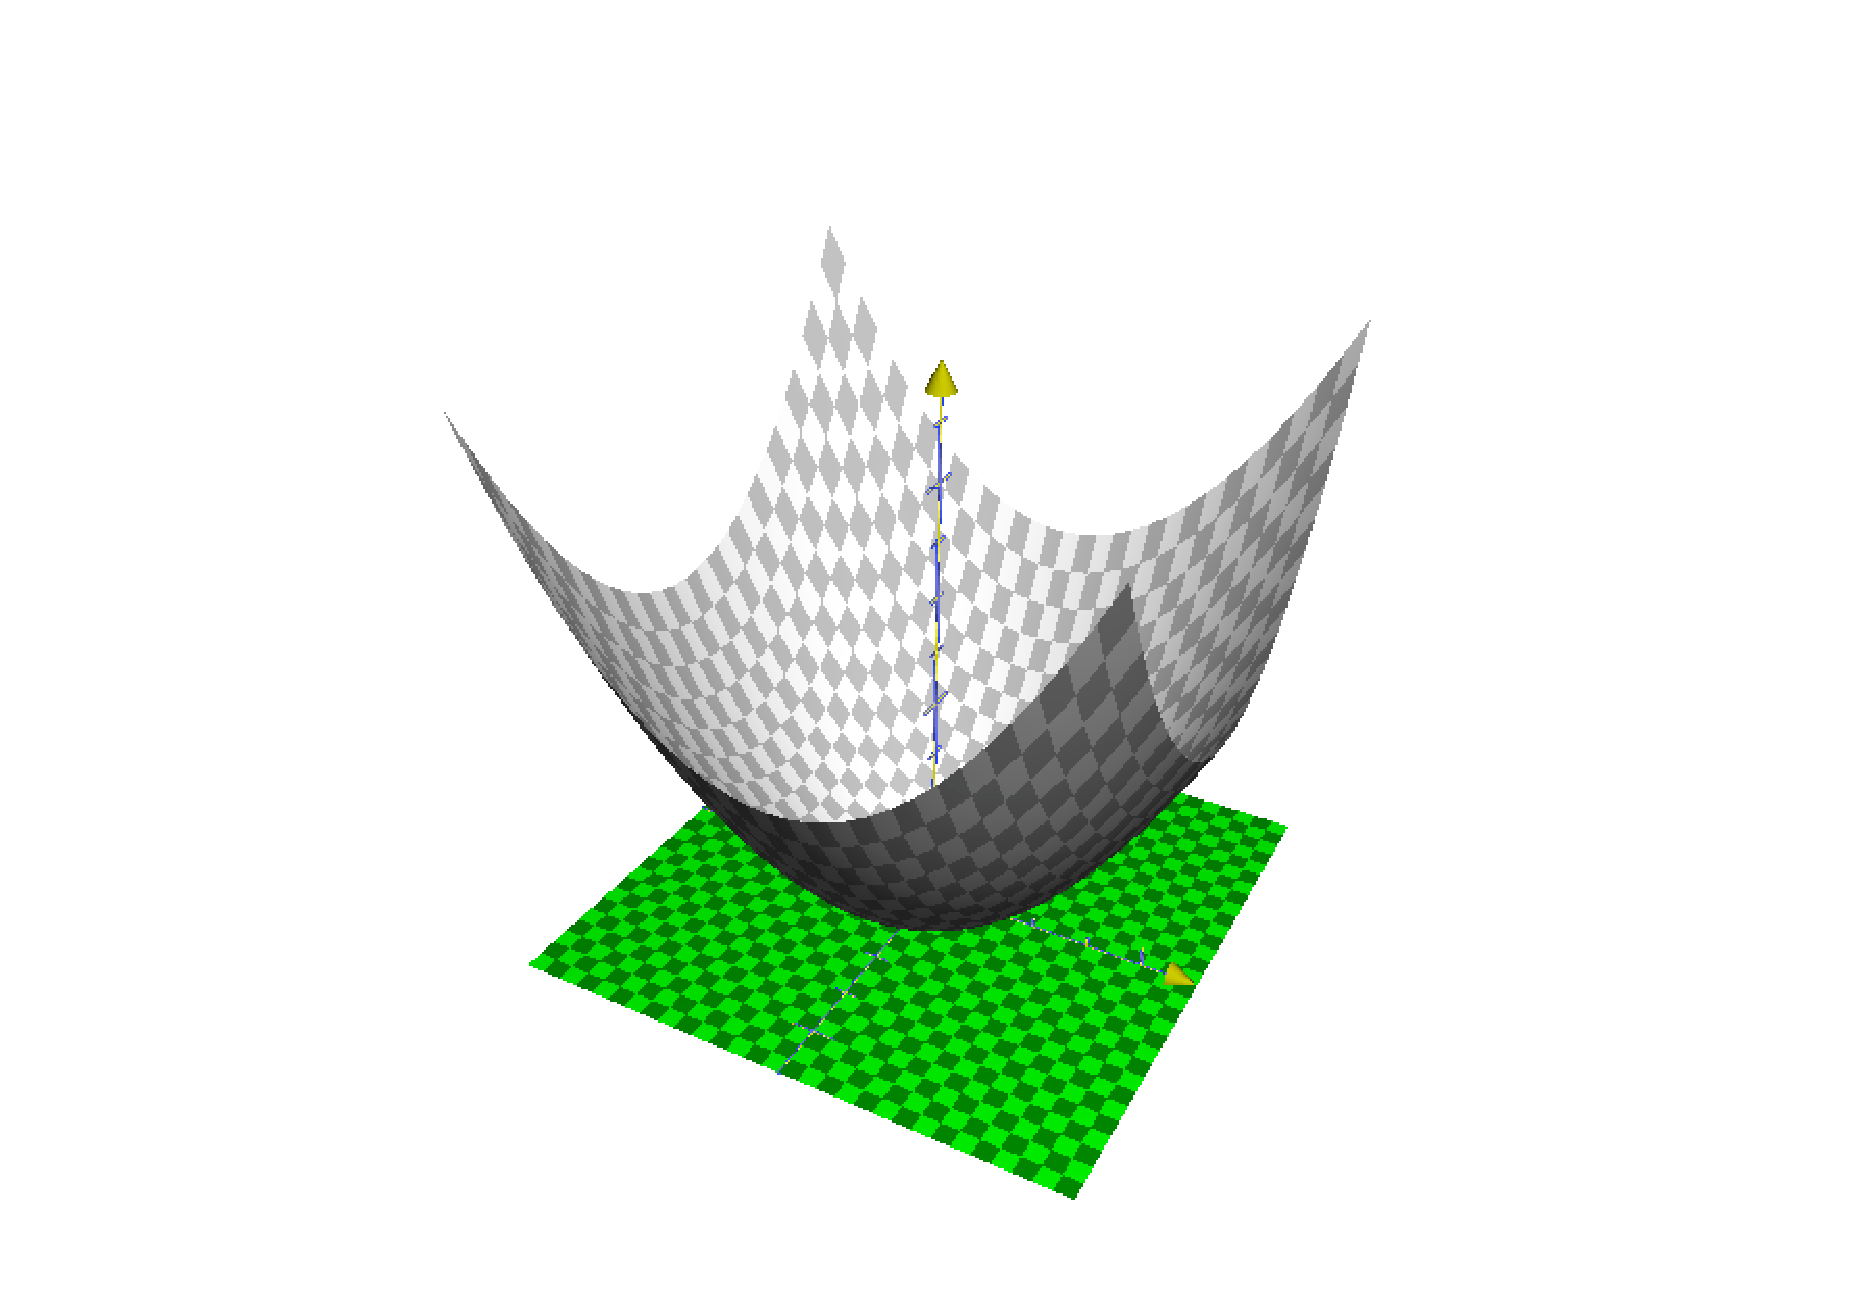
\includegraphics[width=100pt]{03maxmin-on-square3.pdf}
  \caption{The graph of $f(x, y) = x^2+y^2$ from example
    \S~\ref{sec:maxmin-exist-parabolic} on three different rectangles $Q$.
    From left to right:\\
    \null\quad(i) $0\leq x\leq1, 0\leq y\leq1$.
    Both max and min are attained at a corner point of the rectangle.\\
    \null\quad(ii) $0\leq x\leq1, -1\leq y\leq1$. Two maxima, both are attained
    at corner points of the rectangle;
    the minimum is attained at an edge point.\\
    \null\quad(iii) $-1\leq x\leq1, -1\leq y\leq1$, Four maxima, all attained at
    corner points of the rectangle; the minimum is attained at an interior
    point.}
  \label{fig:03maxmin-on-square}
\end{figure}


\label{sec:maxmin-exist-parabolic} 
This function is continuous, and the square $Q = \{(x, y) : 0\leq x\leq1, 0\leq
y\leq1\}$ is bounded, and it contains all boundary points (the edges of the
square).  Therefore Theorem~\ref{thm:maxmin-exist} tells us that $f$ attains
both its highest and lowest values somewhere in the square.  The theorem does
not say where these max/min points are, but in this example they are easy to
find.  The function $f(x, y) = x^2+y^2 $ is at its smallest when both $x=0$ and
$y=0$, i.e.\ at the bottom-left corner of the square.  And $f(x,y)$ is at its
largest when $x$ and $y$ are both as large as they can be, i.e.~when $x=1$ and
$y=1$.  This happens at the top-right corner of the square.

Note that the boundary of the rectangle $Q$ has two different kinds of points:
it has four corner points, and then all the other points that lie on the edges.

If we change the rectangle $Q$ then the minimum can appear at a corner point, a
point on an edge, or in an interior point.  See
Figure~\ref{fig:03maxmin-on-square}.



\subsection{A fishy example}

\label{sec:cubic-maxmin-exist} 
Consider the function $f(x, y) = x^2-x^3-y^2$.  Its zero set is the curve $y^2 =
x^2-x^3$, which is shaped like the letter $\alpha$, or like a fish -- see
Figure~\ref{fig:03maxmin-exist-in-fish}.  The function is positive on the tail
($D_1$) and also on the body ($D_2$) of the fish, it vanishes on the curve that
traces out the fish, and $f$ is negative elsewhere.

We assume that both regions $D_1$ and $D_2$ are closed, which means that we
assume that they include their boundary points. See
Figure~\ref{fig:03maxmin-exist-in-fish} below.

Theorem~\ref{thm:maxmin-exist} does not apply to the region $D_1$ because $D_1$
is not bounded (it contains the whole negative $x$-axis).  But the region $D_2$
is bounded, and our function $f$ is continuous, so
Theorem~\ref{thm:maxmin-exist} does apply to $D_2$.  The theorem tells us that
the function $f$ has a maximal value and a minimal value somewhere in $D_2$.  In
the interior of $D_2$ the function is strictly positive, and at the boundary
points of $D_2$ we have $f=0$.  Therefore each boundary point is a minimum point
of $f$ on $D_2$.  The point(s) in $D_2$ where $f$ attains its highest value must
be somewhere in the interior of $D_2$.  In the next section we will see how to
find it (and how to check that in this case there really only is \emph{one} such
point.)

\begin{figure}[ht]
  \centering
  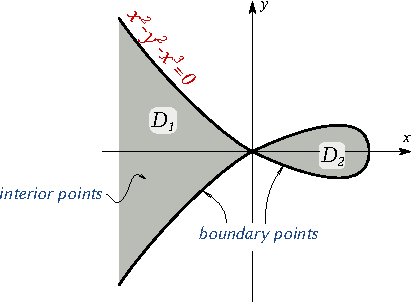
\includegraphics{03maxminexistence.pdf}\hfill
  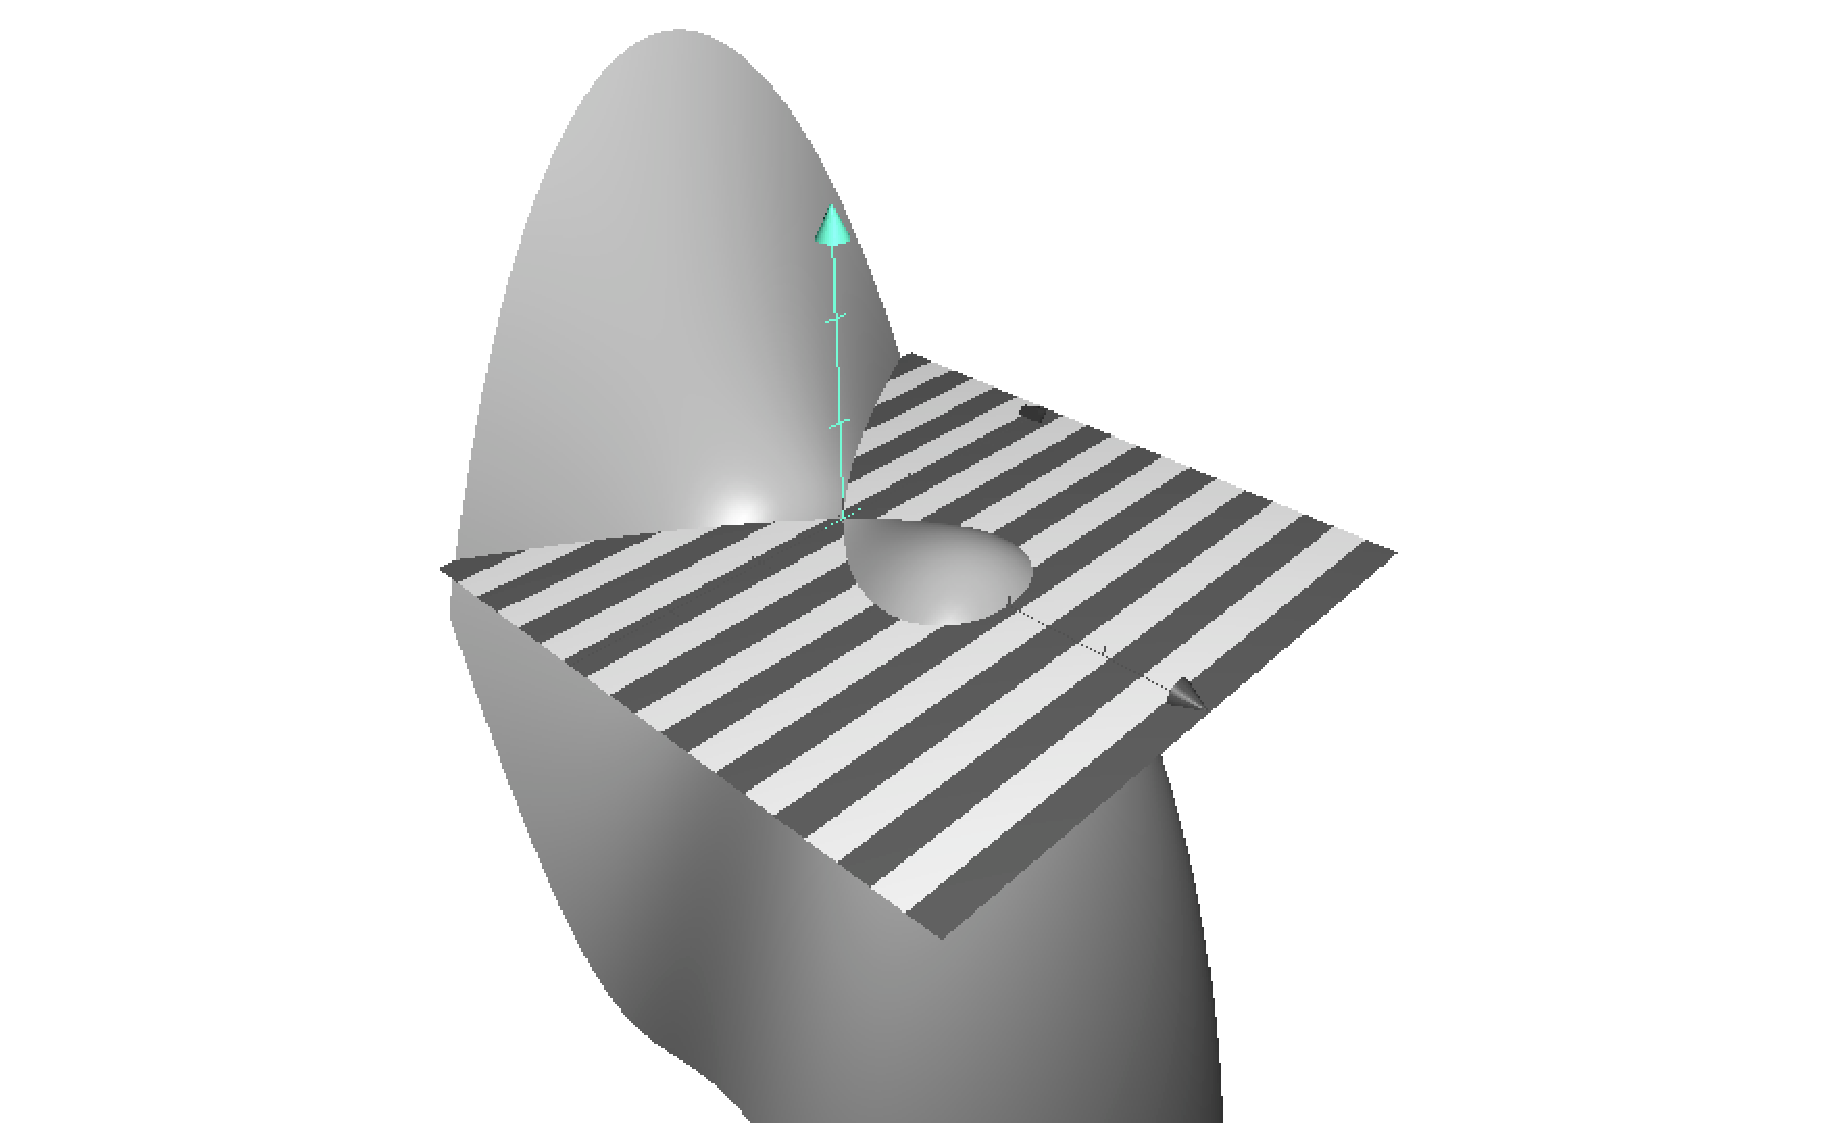
\includegraphics[width=0.3\textwidth]{03maxmin-cubic.pdf}
  
  \caption{ \textbf{Left: } The region where $f(x, y) = x^2-x^3-y^2$ is positive
    consists of two parts, one bounded ($D_2$), and the other unbounded ($D_1$).
    Theorem~\ref{thm:maxmin-exist} does not apply to the unbounded region, but
    it does apply to the bounded region $D_2$. In that region $f$ must attain a
    maximum and also a minimum.  Since $f=0$ on the boundary of the region
    $D_2$, and $f>0$ in the interior, $f$ achieves its lowest value in $D_2$
    everywhere on the boundary of $D_2$ and its highest value somewhere in the
    interior.  Theorem~\ref{thm:maxmin-exist} does not tell us how to find that
    interior point, and allows for the possibility that there might be
    more interior maxima, as well as a few interior (local) minima.\\
    \null\qquad \textbf{Right: } The graph of the function $z=x^2-y^2-x^3$.}
  \label{fig:03maxmin-exist-in-fish}
\end{figure}



\section{Problems}    
\begin{multicols}{2}
\problemfont 

\problem Suppose you want to find the \emph{maximal value} of $f(x, y) =  
x^2-x^3-y^2$ over all possible $(x,y)$ with $x\geq 0$ (and no restriction
on $y$ -- this region is called the \textit{right half plane}).

\subprob Explain why you should always choose $y=0$ in order to 
maximize this particular function $f(x, y)$.
\answer If $y\neq0$ then you can increase $x^2-x^3-y^2$ by setting $y=0$.  
To put it differently, no matter what you choose for $y$, you always have
\[
  f(x, y) = x^2-x^3-y^2 \leq x^2-x^3  =  f(x, 0).
\]
\endanswer

\subprob Use your answer to part \textbf{(a)} to find the point $(x, y)$ that 
maximizes $f(x,y)$ over the right half plane.
\answer 
The maximum has to appear on the $x$ axis, so the question is
\textit{which $x\geq0$ maximizes $f(x, 0) = x^2-x^3$?}

This is a Math~221 question.  The answer is at $x=2/3$.
\endanswer

\subprob Does our function $f(x,y)$ have a maximal value if $(x,y)$ can be 
any point in the plane?  (hint: what is $f(-1000, 0)$?)
\answer  
No, $\lim_{x\to-\infty} f(x, y) = +\infty$, so $f$ has no largest value.
\endanswer

\problem Suppose that $D$ is a bounded and closed region in the plane (you should draw one: any region will do as long as you include the boundary points).

Where does the function $f(x, y)=x$ attain its maximum in the region that you drew?  Can $f$ attain its maximum at an interior point of the region?

What about minima?

\problem Draw the region
\[
R=\left\{ (x,y) : y^2\leq 4(x^3-x^4)  \right\}.
\]
Find the largest and smallest values that the function
$f(x, y) = x$ can have on this region.  

(Hint: where is $4(x^3-x^4) = 4x^3(1-x)$ positive? The region looks like an Onion).
\answer  
\begin{picture} (120.000000,133.111111)(0,0)
    \put(0.0, 0.0){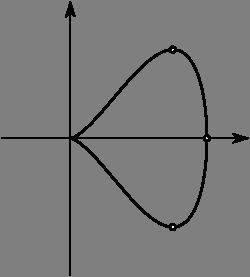
\includegraphics{03onion.pdf}}
        \put(101.33,  68.56){\sffamily\itshape \makebox[0pt][l]{$1$}}
    \put( 82.94, 116.14){\sffamily\itshape \makebox[0pt][c]{$(\frac34, \frac38\sqrt3)$}}
    \put( 82.94,  11.98){\sffamily\itshape \makebox[0pt][c]{$(\frac34, -\frac38\sqrt3)$}}

\end{picture}
%

The quantity $4(x^3-x^4) = 4x^3(1-x)$ is negative when $x<0$ or
$x>1$, so the region is confined to the vertical strip $0\leq x \leq
1$.  Within this strip $R$ is comprised of those points which satisfy
$-\sqrt{4(x^3-x^4)} \leq y \leq +\sqrt{4(x^3-x^4)}$.  The largest
$x$ value is attained at the point with $x=1$, where $y=0$, so, at the
point $(1,0)$.  The smallest $x$ value is attained at the point
$(0,0)$.   The largest $y$ value is attained at the point where
$y^2 = 4x^3-4x^4$ is maximal.  This happens when $x=\frac 34$, and the
largest $y$ value is therefore $\sqrt{4[(3/4)^3-(3/4)^4]} = \frac
38\sqrt{3}$.  The smallest $y$ value also occurs at $x=\frac 34$ and
is given by $y = -\frac 38 \sqrt 3$.
\endanswer

\noproblemfont
\end{multicols}

\section{Critical points}
For functions $y=f(x), a\leq x\leq b$, of one variable the standard way of finding minima (and maxima) is to look for them in two different places: either the minimum is attained at one of the end points $x=a$ or $x=b$ of the interval, or else the minimum is attained at an interior point.  At an interior minimum one has $f'(x) = 0$, so they can be found by solving the equation $f'(x) = 0$.  The same approach works for functions of two or more variables.  The basic fact that tells us that this is so, is the following theorem.

\subsection{Definition (critical point)} \itshape%
A critical point of a function $z=f(x,y)$ of two variables is a point $(a,b)$ at which $\nab f(a,b) = 0$, i.e.~at which
\[
f_x(a,b) = 0 \text{ and } f_y(a,b) = 0.
\]
\upshape

At a critical point of a function the tangent plane to the graph is horizontal.

\subsection{Theorem.  Local extrema are critical points}

\label{sec:extrema-are-critical} 
\itshape If a function $z=f(x,y)$ defined on a domain $D$ has a local minimum or local maximum at an interior point $(a,b)$ then one has
\[
\frac{\pd f}{\pd x}(a,b)=0, \text{ and } \frac{\pd f}{\pd y}(a,b) = 0.
\]
\upshape
\subsubsection*{Picture proof} (See Figure~\ref{fig:max-are-critical-picture-proof}.)  If $f$ has a local maximum at an interior point $(a,b)$ then $f(x, y) \leq f(a, b)$ for all $(x,y)$ close to $(a,b)$.  This means that a small piece of the graph of $f$ near its local maximum at $(a,b,f(a,b))$ lies below the plane $z=f(a,b)$.  This plane must therefore be the tangent plane to the graph of $f$.  Being horizontal, its slopes are zero, and these slopes are exactly the partial derivatives of $f$ at $(a,b)$.

\subsubsection*{Frozen variable proof}
Suppose $f$ has a local maximum at an interior point $(a,b)$ of the domain $D$.  Then we can freeze the $y$-variable at the value $y=b$ and consider the function of one variable $g(x) = f(x,b)$.  This function has a maximum at $x=a$, so by first semester calculus we know that $g'(x) = 0$.  By definition $g'(a) = f_x(x, b)$, so we conclude that $f_x(a,b) = 0$.

By freezing $x$ instead of $y$ we find that $f_y(a,b)=0$ also must hold.

The same arguments apply in the case of a local minimum.
\begin{figure}[htb]
  \centering

  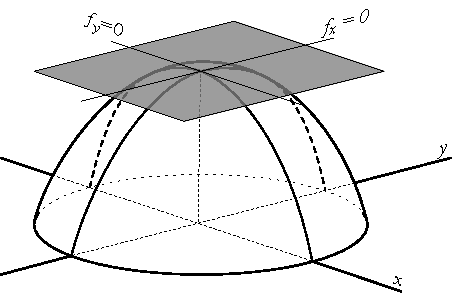
\includegraphics{02localmax.pdf}
  \caption{\textbf{Theorem~\ref{sec:extrema-are-critical}: } at a local maximum the tangent plane to the graph is horizontal.  The partial derivatives w.r.t.\ both $x$ and $y$ vanish, and in fact, the derivative along \emph{any} path through $(a,b)$ vanishes.  To see a picture of a local minimum turn the page upside down.}
  \label{fig:max-are-critical-picture-proof}
\end{figure}

\subsection{Three typical critical points}

\label{sec:criticalpoint-examples} 
Let's find the critical points of the following three functions:
\[
f(x, y) = x^2+y^2, \quad g(x, y) = x^2-y^2, \quad h(x, y) = -x^2-y^2.
\]
\subsubsection*{$\blacktriangleright f(x, y) = x^2+y^2$}
Computing the partial derivatives we find for the first function
\[
\pdd fx = 2x, \quad \pdd fy = 2y.
\]
If $(x,y)$ is a critical point of $f$ then $x$ and $y$ must satisfy the
equations $f_x(x, y) = 0$ and $f_y(x, y) = 0$, in this case, $2x=0$ and $2y=0$.
So we see that $f$ has exactly one critical point, namely the origin $(x,y) =
(0,0)$.

\textit{Is this critical point perhaps a minimum or a maximum?}  Since squares
can never be negative, $f(x,y) = x^2+y^2$ is always non-negative, and it is at
its smallest when both terms $x^2$ and $y^2$ vanish, i.e.~when $x=y=0$.  So
$f(x, y)$ has a global minimum at the origin.

\subsubsection*{$\blacktriangleright h(x, y) = -x^2-y^2$. } 
This function is just $-f(x,y)$, and without looking at its derivatives we can
tell that it has a global maximum at the origin (because $f(x,y)$ has a global
minimum there).  The derivatives are
\[
\pdd hx = -2x, \quad \pdd hy = -2y
\]
so that the origin is the only critical point of this function.

\begin{figure}[htb]
  \centering
  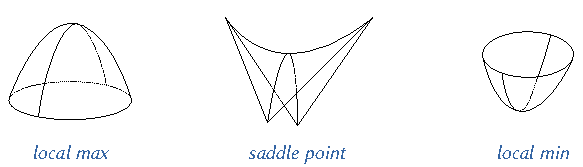
\includegraphics{02threecriticalpoints.pdf}
  \caption{The three most common kinds of critical point.  See the examples in
    \S\ref{sec:criticalpoint-examples} and also the second derivative test in
    \S\ref{sec:second-deriv-test}.}
  \label{fig:most-common-crpts}
\end{figure}

\subsubsection*{$\blacktriangleright g(x, y) = x^2-y^2$. } 
The derivatives of $g$ are
\[
\pdd gx = 2x, \quad \pdd gy = -2y,
\]
so, once again, the origin is the only critical point.  But, unlike the previous
two functions, $g$ has neither a maximum nor a minimum at the origin.  We can
see this by first looking at what $g$ does on the $x$-axis, and then what $g$
does on the $y$-axis:

On the $x$-axis we have $g(x, 0) = +x^2$, so $g$ has a \emph{minimum} at the
origin.

On the $y$-axis we have $g(0,y) = -y^2$, so $g$ has a \emph{maximum} at the
origin.

So arbitrarily close to the origin we can find points $(x,y)$ where $g(x,y)$ is
larger than $g(0,0)$, and we can find other points where $g(x,y)$ is smaller
than $g(0,0)$.  Therefore $g$ does not have a local maximum or a local minimum
at the origin.

Figure~\ref{fig:most-common-crpts} shows the three cases we have just discussed.


\subsection{Critical points in the fishy example}

\label{sec:critical-fish} 
\textit{What are the critical points of the function $f(x, y) = x^2-x^3-y^2$
  from \S \ref{sec:cubic-maxmin-exist}?}

We compute the partial derivatives of the function
\[
\pdd fx = 2x-3x^2 = (2-3x)x,\qquad \pdd fy = -2y.
\]
The equation $f_y=0$ implies that $y=0$, while $f_x=0$ implies $x=0$ or
$x=\frac{2} {3}$.  Therefore $f$ has two critical points: one at the origin
$(0,0)$, and the other at $(\frac23,0)$.

\marginpar{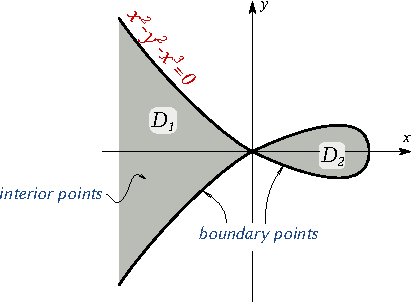
\includegraphics[width=0.25\textwidth] {03maxminexistence.pdf}}

In this example we could have already predicted from the shape of the zero set
of $f$ that $f$ has at least two critical points -- we don't need to compute the
derivatives of $f$ for that.  Namely, the zero set of $f$ is a curve that
crosses itself at the origin, so the Implicit Function
Theorem~\ref{thm:01implicit-function} (chapter 2) cannot hold at the origin, and
hence $f_x=f_y=0$ there.  And in \S~\ref{sec:cubic-maxmin-exist} we argued that
the function $f$ must have a local maximum somewhere in the region $D_2$
(Figure~\ref{fig:03maxmin-exist-in-fish}), so $f$ must have at least two
critical points.  On the other hand, by computing the critical points we have
found that there is only one local maximum in the region $D_2$.


\subsection{Another example -- find the critical points of $f(x,y) =x-x^3-xy^2$}

\subsubsection*{Solution: } The derivatives of our function are
\[
\pdd fx = 1-3x^2-y^2,\qquad \pdd fy = -2xy.
\]
The critical points are therefore the solutions of the equations
\[
1-3x^2-y^2=0,\qquad -2xy=0.
\]
This is a system of two equations, with two unknowns (that always happens when
we look for critical points, since we are looking for solutions of $f_x(x,y) =
0$, $f_y(x,y)=0$.)  The second equation, $-2xy=0$, implies that either $x=0$ or
$y=0$ (or both).  We have to treat these two cases separately:
\begin{quote}
  \begin{trivlist}
  \item [\bf The case $x=0$. ] If $x=0$ then we only have the first equation
    left, which tells us $1-y^2=0$, i.e.\ $y=\pm1$.  We find two critical points
    with $x=0$, namely, $(0,1)$ and $(0,-1)$.
  \item [\bf The other case, $x\neq0$. ] If $x\neq0$, then the second equation
    ($-2xy=0$) implies $y=0$.  Substitute this in the first equation and we find
    $1-3x^2=0$, i.e.\ $x=\pm\frac{1} {3}\sqrt{3}$, so that we have two critical
    points with $x\neq0$, namely, $(-\frac13\sqrt3, 0)$ and $(\frac13\sqrt3,
    0)$.
  \end{trivlist}
\end{quote}

\begin{figure}[h]
  \centering
  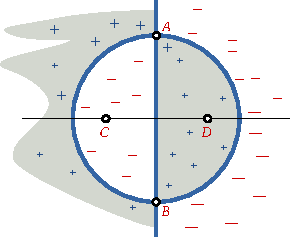
\includegraphics{03example-criticalpoints.pdf}
  \caption{The zero set and signs of the function $f(x,y) =x-x^3-xy^2$.}
  \label{fig:circle-and-line-zero-set-example}
\end{figure}


The conclusion is that this function has four critical points, two on the
$x$-axis, and two on the $y$-axis.  Without looking into this in any further
detail we cannot tell if any of these points are local maxima or minima.  In
general the second derivative test (to be explained in
\S~\ref{sec:second-deriv-test}) will provide this information.  For this example
a look at the zero set of $f$ also helps us figure out what kind of critical
points we have found.  Since $f$ factors as
\[
f(x, y) = x\cdot (1-x^2-y^2),
\]
we see that its zero set consists of the line $x=0$ and the unit circle
$x^2+y^2=1$.  In the above picture $f>0$ in the grey region, and $f<0$ in the
white area.  Consider the right half of the unit disc.  The function is positive
in the interior, and zero on the boundary of this region.  Just as in the
``fishy example'' of \S~\ref{sec:cubic-maxmin-exist}, we have another case where
the maximum of the function must be attained at one or more interior points of
the right half of the unit disc.  According to our computation $f$ only has
\textit{one} critical point in the right half circle, and therefore this point
must be a local maximum of the function.  Conclusion: $D=(\frac13\sqrt3,0)$ is a
local maximum.

In the same spirit you can argue that $f$ has a local minimum at $C$.

The other two points $A,B$ are neither local maxima nor minima, since
\textit{arbitrarily close to $A$ or $B$} there are both points $(x,y)$ with
$f(x,y)$ positive, and points with $f(x,y)$ negative.  The points $A$ and $B$
turn out to be ``saddle points'' (see \S\ref{sec:second-deriv-test} on the
second derivative test.)

\section{When there are more than two variables}
The whole discussion so far has been about functions of two variables.
Fortunately, not much changes when you have more variables.  The concepts
\textit{local minimum} and \textit{local maximum} are defined in the same way,
and it turns out that any \textit{interior local maximum or minimum must be a
  critical point of the function}.  Here, by definition, a critical point of a
function $w=f(x_1, \ldots, x_n)$ of $n$ variables is a solution of the equations
\[
\left\{
  \begin{gathered}
    \pdd f{x_1} (x_1, \cdots, x_n) =0\\
    \pdd f{x_2} (x_1, \cdots, x_n) =0\\
    \vdots\\
    \pdd f{x_n} (x_1, \cdots, x_n) =0.
  \end{gathered}
\right.
\]
Observe that there are $n$ equations, and that there are also $n$ unknowns
($x_1$, \ldots, $x_n$) so that we should \textit{in principle} be able to solve
these equations.  In practice the system of equations we get can be very easy,
difficult, or simply impossible to solve.

\newpage
\section{Problems}  
\begin{multicols}{2}
\problemfont
\problem\label{prb:find-critical-points}  
Find all critical points of the following functions.  Try to classify
them into local/global maxima/minima, saddles, or other kind of
critical points.  (Write clear solutions.  You will need your
solutions later in problem \ref{prb:lots-of-2nd-deriv-tests}.)

\subprob $f(x,y)=x^2+4y^2-2x+8y-1$
%
\answer 
$f_x = 2x-2$, $f_y = 8y+8$, $f_{xx} = 2$, $f_{xy}=0$, $f_{yy}=8$.

There is exactly one critical point, at $(x, y) = (1,-1)$.

The 2nd order Taylor expansion at this point is 
\[
f(1+\Delta x, -1+\Delta y) = 
f(1, -1) + (\Delta x)^2 + 4(\Delta y)^2 +\cdots
\]
The quadratic part is positive definite, therefore $f$ has a
\emph{local minimum} at $(1, -1)$.
\endanswer

\subprob $f(x,y)=x^2-y^2+6x-10y+2$ 
%
\answer 
$f_x = 2x+6$, $f_y = -2y-10$, $f_{xx} = 2$, $f_{xy}=0$, $f_{yy}=-2$.

There is exactly one critical point, at $(x, y) = (-3,-5)$.

The 2nd order Taylor expansion at this point is 
\begin{align*}
  f(-3+\Delta x, -5+\Delta y)
  &= f(-3, -5) + (\Delta x)^2 - (\Delta y)^2 +\cdots \\
  &= f(-3, -5) +\bigl(\Delta x-\Delta y\bigr)\bigl(\Delta x +\Delta
  y\bigr)+\cdots
\end{align*}
The quadratic part factors, therefore $f$ has a
\emph{saddle point} at $(-3, -5)$.  The level set near the critical
point consists of two crossing curves whose tangents are given by the
equations $\Delta x=\Delta y$ and $\Delta x=-\Delta y$.  Since
$\Delta x=x-a=x+3$ and $\Delta y = y-b = y+5$, the two tangent lines
have equations $x+3 = y+5$ and $x+3 = -(y+5)$.
\marginpar{\footnotesize\sffamily
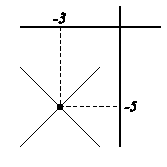
\includegraphics{03answers001.pdf}
\\
Critical point and level set near the critical point.
}%

\endanswer

\subprob $f(x,y)=x^2+4xy+y^2-6y+1$ 
\label{prb:find-cpt-01}
\answer 
$f_x = 2x+4y$, $f_y = 4x+2y$, $f_{xx} = 2$, $f_{xy}=4$, $f_{yy}=2$.
There is one critical point: $(x,y) = (2, -1)$.

The 2nd order Taylor expansion at this point is 
\begin{align*}
f(2+\Delta x, -1+\Delta y)
&= f(2, -1) + (\Delta x)^2 + 4 \Delta x \Delta x
            + (\Delta y)^2 +\cdots\\
&= f(2, -1) + \bigl(\Delta x+2\Delta y\bigr)^{2}
            - 3(\Delta y)^2+\cdots\\
&= f(2, -1) + \bigl(\Delta x+(2+\surd3)\Delta y\bigr)
              \bigl(\Delta x+(2-\surd3)\Delta y\bigr)
            +\cdots
\end{align*}
\marginpar{\footnotesize\sffamily
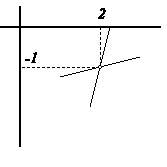
\includegraphics{03answers002.pdf}
\\
Critical point and level set near the critical point.
}%
The quadratic part factors, therefore $f$ has a
\emph{saddle point} at $(2, -1)$.  The level set near the critical
point consists of two crossing curves whose tangents are given by the
equations $\Delta x=-(2+\surd 3)\Delta y$ and $\Delta x=-(2-\surd
3)\Delta y$.  Since $\Delta x=x-a=x-2$ and $\Delta y = y-b = y+1$, the
two tangent lines have equations $x-2 = -(2+\surd3)(y+1)$ and
$x-2 = -(2-\surd3)(y+1)$.
\endanswer

\subprob  $f(x,y)=$\\
\null\hfill$x^2-xy+2y^2-5x+6y-9$ 
\label{prb:find-cpt-02}
\answer 
$f_x = 2x-y-5$, $f_y = -x+4y+6$, $f_{xx} = 2$, $f_{xy}=-1$, $f_{yy}=4$.

There is again one critical point: $x=2$, $y=-1$.

The 2nd order Taylor expansion at this point is 
\begin{align*}
f(2+\Delta x, -1+\Delta y)
&= f(2, -1) + (\Delta x)^2 - \Delta x \Delta x
            + 2(\Delta y)^2 +\cdots\\
&= f(2, -1) + \bigl(\Delta x-\tfrac12\Delta y\bigr)^{2}
            +\tfrac74(\Delta y)^2+\cdots
\end{align*}
The second order part of the Taylor expansion is positive, so
$(2, -1)$ is a \emph{local minimum}.

\endanswer

\subprob $f(x,y) = y^2-18 x^2+x^4$ 
\answer   
$f_x = -36x+4x^3$, $f_y = 2y$, $f_{xx} = -36+12x^2$, $f_{xy}=0$,
$f_{yy}=2$.

The equation $f_x=0$ has three solutions, $x=0$ and $x=\pm3$.
The equation $f_y=0$ has only one solution $y=0$.
Therefore there are three critical points, the origin and the points
$(\pm 3,0)$.

The taylor expansions at these points are
\begin{align*}
    f(\Delta x, \Delta y) 
    &= f(0,0) -18 (\Delta x)^2 + (\Delta y)^2 + \cdots \\
    &= f(0,0) + \bigl(\Delta y-\sqrt{18} x\bigr)\bigl(\Delta y+\sqrt{18} x\bigr)
              + \cdots \\
    f(3+\Delta x, \Delta y) 
    &= f(3,0) +36 (\Delta x)^2 + (\Delta y)^2 + \cdots \\
    f(-3+\Delta x, \Delta y) 
    &= f(-3,0) +36 (\Delta x)^2 + (\Delta y)^2 + \cdots 
\end{align*}
The second order terms in the Taylor expansions at $(3,0)$ and at
$(-3,0)$ are both positive for all $\Delta x$ and $\Delta y$, so both
points $(\pm3, 0)$ are local minima.  The second order part of the
expansion at the origin factors and hence the origin is a saddle
point.  The tangents to the zeroset at the origin are the lines
$\Delta y = \pm \sqrt{18}\Delta x = \pm 3\sqrt2 \Delta x$.  Since here
$\Delta x = \text{``}x-a\text{''} = x$, and $\Delta y = y$, the
tangents are the lines through the origin given by $y=\pm 3\sqrt2 x$.

You can try to draw the zeroset of this function and analyze it in the
same way as the ``fishy example'' in \ref{sec:critical-fish}.  The
zeroset of $f$ consists of the graphs of $y = \pm \sqrt{18x^2-x^4} =
\pm |x|\sqrt{18-x^2}$.
It looks like a squashed ``$\infty$'' or a butterfly (you decide.)
\marginpar{\footnotesize\sffamily
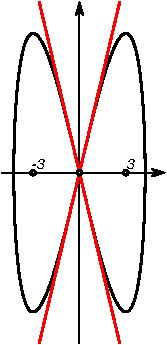
\includegraphics{03answers003.pdf}
\\
Critical points and zero set.
}
\endanswer
\subprob $f(x,y) = y^4-4y^2-18 x^2+x^4$ 
%
\answer    
There are nine critical points. Four global minima at $(\pm 3,
\pm\sqrt{3})$, four saddle points at $(0,\pm\sqrt{3})$ and $(\pm3,0)$
respectively, and finally, a local but not global maximum at the
origin.
\endanswer

\subprob $f(x,y)=9+4x-y-2x^2-3y^2$ 
%
\answer critical point at $(1,-1/6)$  
$f_x = 4-4x$, $f_y = -1-6y$, $f_{xx} = -4$, $f_{xy}=0$, $f_{yy}=-6$.

Second order Taylor expansion at the critical point:
\[
f(-1+\Delta x, -\tfrac16+\Delta y) = f(1, -\tfrac16)
-2(\Delta x)^2-3(\Delta y)^2 + \cdots
\]
The second order terms are always negative so $(1, -\tfrac16)$ is a
local maximum.
\endanswer

\subprob $f(x,y)=xy(4-x-2y)$ 
%
\answer The derivatives are: 
\[
f_x = 4y-2xy-2y^2,\quad f_y = 4x-x^2-4xy,\quad f_{xx} = -2y,\quad
f_{xy}=4-2x-4y,\quad f_{yy}=-4x.
\]
This function is given in factored form, so without solving the
equations $f_x=0$, $f_y=0$ you can say the following about this
problem.  The zero set consists of the three lines: the $y$-axis
($x=0$), the $x$-axis ($y=0$) and the line with equation $4-x-2y=0$.
It follows that the intersection points $(0,0)$, $(4,0)$, and $(0,2)$
of these lines are saddle points.  Since $f>0$ in the triangle formed
by the three lines this triangle must contain at least one local
maximum.

\begin{center}
  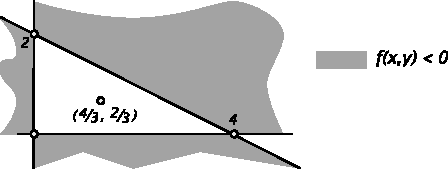
\includegraphics{03answers004.pdf}
\end{center}
To find all critical points solve these equations:
\[
f_x = 4y-2xy-2y^2 = 0 \iff \text{\framebox{$y=0$ or $4-2x-2y=0$}}
\]
and 
\[
f_y = 4x-x^2-4xy=0  \iff \text{\framebox{$x=0$ or $4-x-4y=0$}}
\]
Since both equations $f_x=0$ and $f_y=0$ lead to two possibilities, we
have to consider $2\times 2=4$ cases:
\begin{description}
  \item[$y=0$ \& $x=0$] This tells us the origin is a critical point
  \item[$y=0$ \& $4-x-4y=0$] Solving these equations leads to
    $x=4, y=0$, so $(4,0)$ is a critical point.
  \item[$4-2x-2y=0$ \& $x=0$] Solve and you find that $(0,2)$ is a
    critical point.
  \item[$4-2x-2y=0$ \& $4-x-4y=0$] Solve these equations and you get
    $(x,y) = (\tfrac43, \tfrac23)$.
\end{description}
The first three critical points are the saddle points we predicted.
The fourth critical point must be a local maximum, since there has to
be one in the triangle, and of all the critical points we have found
the others are all saddle points.
\endanswer

\subprob $f(x,y)=x(x-y)(x-1)$ 
\answer
Two saddle points:  $(0,0)$ and $(1,1)$.
\endanswer

\subprob $f(x,y)=(x-y)(xy-4)$ 
%
\answer Two saddle points:  $(2,2)$ and $(-2,-2)$  
%$f_x = <++>$, $f_y = <++>$, $f_{xx} = <++>$, $f_{xy}=<++>$, $f_{yy}=<++>$.
\endanswer

\subprob $f(x,y)=y^2+\cos x$ 
%
%\answer    
%$f_x = <++>$, $f_y = <++>$, $f_{xx} = <++>$, $f_{xy}=<++>$, $f_{yy}=<++>$.
%\endanswer

\subprob $f(x,y)=x^2y-\frac13 y^3$ 
%
\answer The origin. Neither a local max, min, nor saddle.  
The graph of this function is called the ``Monkey Saddle'' as
it accommodates two legs and a tail too.  Draw it in your graphing
program to see this.
\endanswer

\subprob $f(x,y)=(x-y^2)(x-1)$ 
%
\answer    
Zero set is the parabola with equation $x=y^2$, and the line
$x=1$.  They intersect at $(1, \pm1)$, so the function has two saddle
points $(1,1)$ and $(1,-1)$.  The region between the line $x=1$ and
the parabola must contain  local minimum.  It is located at
$(\frac12, 0)$.
\endanswer

\subprob $f(x,y)=(x-y)(xy-4)$ 
%
\answer Two saddle points : $(2,2)$ and $(-2,-2)$.  
Yes, this problem appeared twice.
\endanswer

\subprob $f(x,y) = x^2$ 
%
\answer  All points on the $y$-axis are critical points.  They are all  
global minima, but the second derivative test doesn't tell you so.
\endanswer

\subprob $f(x,y) = x^2y$ 
%
\answer  
All points on the $y$-axis are again critical points.  Those with
$y>0$ are local minima, those with $y<0$ are local maxima, and the
origin is neither.  The second derivative test applies to none of
these points.
\endanswer

\subprob $f(x,y) = \bigl(1-x^2-y^2\bigr)^2$ 
%
\answer  All points on the unit circle are global minima, because the  
function vanishes there, and is positive everywhere else.  The origin
is a local maximum.  The 2nd derivative test applies to the origin,
but not to any of the other critical points.
\endanswer

\subprob $f(x,y) = x^2y$ 
%
\answer  
All points on the $y$-axis are again critical points.  Those with
$y>0$ are local minima, those with $y<0$ are local maxima, and the
origin is neither.  The second derivative test applies to none of
these points.
\endanswer

\problem % about f(x, y) = sin x sin y    

\subprob Draw the zero set of the function $f(x, y) = \sin(x) \sin(y)$.

\subprob Where is the function $f$ positive?  Find as many critical points as
you can without computing $f_x$ or $f_y$.

\subprob Find all critical points of $f(x, y)$.  Which are local minima or local
maxima?

\problem Find the critical points of the function 
\[
f(x, y, z) = x^2 + y^2 + z^2 - 2x + 4y -2.
\]

\problem Draw the zero set and find the critical points of the functions
\[
f(x, y, z) = x^2+y^2 - z^2
\]
and
\[
g(x, y, z) = x^2-y^2 - z^2
\]

\problem If we have three points $A$,  $B$, and $C$ in the plane, \textit{which point is closest to all three of them?}  The answer depends on what we mean by ``closest to all three points.''  The following problem gives us one interpretation of this general question.

Consider the three points $(1,4)$, $(5,2)$, and $(3,-2)$ in the plane.  The function 
\begin{multline*}
f(x, y, z) = \\
(x-1)^2+(y-4)^2+\\
(x-5)^2+(y-2)^2+\\
(x-3)^2+(y+2)^2
\end{multline*}
is the sum of the squares of the distances from point $(x,y)$ to the
three points.  

\subprob Assuming that there is a global minimum, find $x$ and $y$ so that $f(x,y)$  is minimized. 
\answer  $(3,4/3)$  
\endanswer

\subprob (For discussion)  Does $f(x,y)$ have a global minimum?  How can we be sure
that the point we found in part \textbf{(a)} is not actually a maximum or some other
critical point?
%
\subprob Given the three points $(a, b)$, $(c, d)$, and $(e, f)$,  
let $f(x, y)$ be the sum of the squares of the distances from point
$(x,y)$ to the three points.  Find $x$ and $y$ so that this quantity is
minimized. 
\answer
$x= (a+c+e)/3$, $y=(b+d+f)/3$.  
\endanswer

\problem Suppose that a function $f(x, y)$ factors, i.e.~we can write it as the
product of two other differentiable functions, $f(x, y) = g(x, y)h(x, y)$.

\textit{Prove: if a point $(a, b)$ lies in the zero set of $g$ and also in the
zero set of $h$, then $(a,b)$ is a critical point of $f$.}

\noindent%
Hint: compute the partial derivatives of $f$ by applying the product rule to $f=g\cdot h$.
\answer
You have to show that $f_x(a, b) = f_y(a, b) = 0$.
By the product rule $f_x(a, b) = g_x(a, b)h(a, b) + g(a, b) h_x(a,
b)$.  Since both $g(a, b) = 0$ and $h(a, b) = 0$, it follows that
$f_x(a, b) = 0$.   The same reasoning applies to $f_y(a, b)$.
\endanswer

\problem Find the critical points of the functions 

\subprob $  f(x, y, z) = x^2 + y^2 + z^2 - 2x + 4y -2$ 

\subprob $  f(x, y, z) = x^4 + y^2 + z^2 - 2xz + 4y$ \\

\subprob $  f(x, y, z) = xyze^{-x-y-z}$ 

\subprob $f(x,y,z) = x^2+y^2+z^2 - 2xyz$ 



\noproblemfont
\end{multicols}
\section{A Minimization Problem: Linear Regression}

\label{sec:linear-regression}

Suppose we are measuring two quantities $x$ and $y$ in some experiment, and
suppose that we expect that there is a linear relation of the form $y=ax+b$
between $x$ and $y$.  If we have a set of data points $(x_k, y_k)$ from our
experiment, then what do they tell us about $a$ and $b$?  \emph{Which choice of
  coefficients $a$ and $b$ bests fits our data? } Because of experimental errors
we would not expect our data points to lie on a straight line, but instead, we
expect them to be clustered around a straight line.  We could plot the data
points, get a ruler, and draw a straight line by hand that looks like the best
match -- then we could measure $a,b$ from our drawing.  A more systematic
approach is to first define what we mean by ``best match'' and then find the
line that best matches according to our chosen criterion.

A very common criterion is the least-mean-square-fit.  To describe it, imagine
we have $N$ data points, $(x_1,y_1)$, \dots\, , $(x_N, y_N)$, and consider the
line with coefficients $a$ and $b$.  Most data points $(x_k, y_k)$ will then
probably not lie on the line $y=ax+b$, and one uses
\[
E_k = \tfrac12\bigl(ax_k+b-y_k\bigr)^2
\]
as a measure for the mismatch between the data point $(x_k, y_k)$ and the line
$y=ax+b$ (the factor $\frac12$ makes formulas later on nicer).  Adding all these
errors we get the total ``mean square'' error
\[
E= E_1 + \cdots + E_N.
\]
If we think of all the numbers $x_1, \ldots, x_N, y_1, \ldots, y_N$ as given
constants (after all, we measured them, so we shouldn't change them any
more\footnote{This is called the ``Sushi Principle'': \textit{raw data is better
    than cooked data.}}), then the total error only depends on the coefficients
$a$ and $b$.  It is a measure for how well the line $y=ax+b$ fits our data
points, and the common method of \emph{linear regression} consists in choosing
the coefficients $a$ and $b$ so as to minimize this error $E$.

\begin{figure}[htb]
  \centering \begin{picture} (300.000000,162.461538)(0,0)
    \put(0.0, 0.0){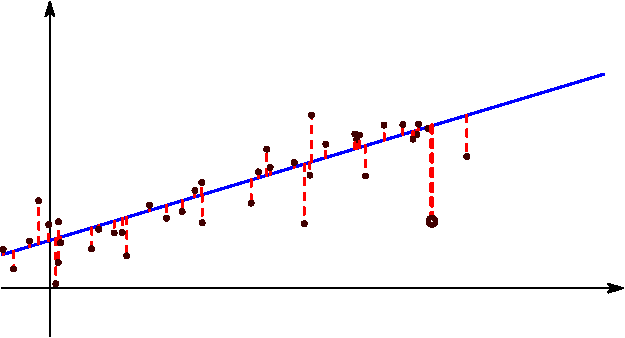
\includegraphics{02linearregression.pdf}}
        \put(241.69, 116.18){\sffamily\itshape \makebox[0pt][l]{\rotatebox{16.699244}{$y=ax+b$}}}
    \put(207.31,  46.02){\sffamily\itshape \makebox[0pt][c]{$(x_k, y_k)$}}
    \put(211.31,  78.94){\sffamily\itshape \makebox[0pt][l]{$\bigl|ax_k+b-y_k\bigr|$}}

\end{picture}

  \caption{Which line best fits a set of data points?}
  \label{fig:linear-regression}
\end{figure}

This leads us to the problem of finding the critical points of the total error
$E$ as a function of $a$ and $b$.  We have to solve
\[
\pdd Ea = 0 \qquad \pdd Eb = 0.
\]
The total error is the sum of the individual errors $E_k(a, b)$ so we get
\[
\pdd Ea = \pdd{E_1}a + \cdots +\pdd {E_N}a, \qquad \pdd Eb = \pdd{E_1}b + \cdots
+\pdd {E_N}b.
\]
The individual errors have the following derivatives:
\[
\pdd{E_k}a = x_k\bigl(ax_k+b-y_k\bigr),\qquad \pdd{E_k}b = ax_k+b-y_k.
\]
Adding all these derivatives then leads to
\begin{align*}
  \pdd Ea &= \sum x_k\bigl(ax_k+b-y_k\bigr) \\
  &= (\tsum x_k^2) a + (\tsum x_k) b - \tsum x_ky_k
\end{align*}
and
\begin{align*}
  \pdd Eb &= \sum \bigl\{ax_k+b-y_k\bigr\} \\
  &= (\tsum x_k) a + N b - \tsum y_k
\end{align*}
Here ``$\sum$'' represents summation over $k=1, \cdots, N$, i.e.\ $\sum x_ky_k =
x_1y_1+\cdots+x_Ny_N$, etc.

If $(a,b)$ is a critical point then $a$ and $b$ must satisfy
\begin{align*}
  (\tsum x_k^2) a + (\tsum x_k) b &= \tsum x_ky_k \\
  (\tsum x_k) a + N b &= \tsum y_k
\end{align*}
These are two linear equations for the two unknowns $a$ and $b$.  Solving them
leads to
\[
a = \frac{N\sum x_ky_k \; - \; \sum x_k \sum y_k} {N\sum x_k^2 - \bigl(\sum
  x_k\bigr)^2}\; ; \qquad b = \frac{-\sum x_k \sum x_ky_k + \sum x_k^2 \sum y_k}
{N\sum x_k^2 - \bigl(\sum x_k\bigr)^2}\; .
\]
These are the standard formulas for the coefficients $a$ and $b$ provided by the
method of linear regression.  Most calculators, and certainly all spreadsheets
(like Excel) have these formulas preprogrammed, so we only have to enter the
data points $(x_k,y_k)$ and ``push the right button'' to get $a$ and $b$.

\section{Problems} 
\begin{multicols}{2}
\problemfont
%\immediate\write\ans{\string\newpage}
\problem  We are given $N$ measurements $x_1$, \ldots, $x_N$  
from some experiment, and, inspired by the Linear Regression example,
we decide to see which number $a$ ``best fits the data.''  We define
the error (or ``measure of misfit'') for each measurement to be
\[
E_k(a) = \tfrac12(a-x_k)^2
\]
and we look for the number $a$ which minimizes the total error
\[
E(a) = E_1(a) + \cdots + E_N(a).
\]
\subprob  Is this a problem about several variable calculus, or about 
one variable calculus?
\answer  
One variable calculus!  There is only one variable, $a$, and we must
solve $E'(a) = 0$.
\endanswer

\subprob Which number $a$ do we find? 
\answer  
$a= (x_1+\cdots+x_N)/N$, i.e.\ the average provides ``the best fit.''
\endanswer

\problem We have a series of data points $(x_k, y_k)$,  
and when we plot them we think we see a convex curve rather than a
straight line.  In fact it looks like a parabola, and so we
set out to find a quadratic function $y=ax^2+bx+c$ that minimizes the
error
\[
E(a,b,c)=E_1+\cdots+E_N,
\]
with
\[
E_k(a, b, c) = \tfrac12\bigl(ax_k^2+bx_k+c - y_k\bigr)^2.
\]
\subprob How many variables are there in this problem? 
\answer Three:  $a$, $b$, and $c$. 
\endanswer
\subprob If $(a, b, c)$ is a critical point of $E(a, b, c)$  
then $a$, $b$, and $c$ satisfy three linear equations.  Find these
equations (don't solve them).
\answer The equations for $(a, b, c)$ are:   
\[
\begin{array}{rlcrlcrlrcl}
    (\tsum x_k^4)&a &+&(\tsum x_k^3)&b &+& (\tsum x_k^2)&c 
    &=& \tsum x_k^2y_k\\[1ex]
    (\tsum x_k^3)&a &+&(\tsum x_k^2)&b &+& (\tsum x_k)&c 
    &=& \tsum x_ky_k\\[1ex]
    (\tsum x_k^2)&a &+&(\tsum x_k)&b &+& N&c &=& \tsum y_k
\end{array}
\]
\endanswer

\problem A measurement in a certain experiment results 
in three numbers $(x, y, z)$.  The point of the experiment is to see
if there is a linear relation of the form $z=ax+by+c$ between the
three measured quantities, and to estimate the coefficients $a, b, c$.

After repeating the experiment $N$ times we have $N$ data points
$(x_k, y_k, z_k)$ ($k=1, \ldots, N$).  We decide to choose $a,b,c$ so
as to minimize the mean square error
\[
E=E_1+\cdots+E_N,
\]
with
\[
E_k(a, b, c) = \tfrac 12 \bigl(ax_k+by_k+c- z_k\bigr)^2.
\]
Which (linear) equations will we get for $a$, $b$, and $c$?
\answer The equations are 
\[
\begin{array}{rlcrlcrlrcl}
    (\tsum x_k^2)&a &+&(\tsum x_ky_k)&b &+& (\tsum x_k)&c 
    &=& \tsum x_kz_k\\[1ex]
    (\tsum x_ky_k)&a &+&(\tsum y_k^2)&b &+& (\tsum y_k)&c 
    &=& \tsum y_kz_k\\[1ex]
    (\tsum x_k)&a &+&(\tsum y_k)&b &+& N&c &=& \tsum z_k
\end{array}
\]
\endanswer
\noproblemfont
\end{multicols}

\section{The Second Derivative Test}    
\label{sec:second-deriv-test}

\subsection{Review of the one-variable second derivative test and Taylor's formula}
For a function $y=f(x)$ of one variable you can tell if a critical
point $a$ is a local maximum or minimum by looking at the sign of the
second derivative $f''(a)$ of the function at that point.  

\begin{figure}[ht]\centering
  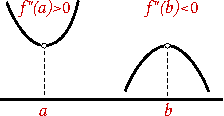
\includegraphics{03onevariable-2ndderivtest.pdf}
\end{figure}
If $f''(a)>0$ then the graph of $f$ is curved upwards and $f$ has a local
minimum at $a$; if $f''(a)<0$ then $f$ has a local max.  This section
is about the analogous test for critical points of functions of two
variables.  

One way to understand the second derivative test is to look at the
Taylor expansion of the function $y=f(x)$.  If $x=a$ is a critical
point for $f$, then
\[
f(x) = f(a) + f'(a)(x-a) + \tfrac 12 f''(a)(x-a)^2
+\cdots
\]
Since $a$ is a critical point of $f$ we have $f'(a)=0$, so that the
Taylor expansion reduces to
\begin{equation}\label{eq:one-variable-expansion-at-cpt}
  f(x) = f(a) + \tfrac 12 f''(a)(x-a)^2 +\cdots
\end{equation}
If we ignore the remainder term (the dots), then we find that
\[
f(x) \approx f(a) + \tfrac 12 f''(a)(x-a)^2.
\]
Near the critical point the graph of $y=f(x)$ is a approximately a
parabola. It is curved upwards if $f''(a)>0$, and downwards if
$f''(a)<0$.

To apply the same reasoning to a function of two (or more) variables
we need to know the Taylor expansion of such a function.

\subsection{Taylor's formula for a function of several variables}
\label{sec:Taylor-derived}
The Taylor expansion of a function $z=f(x, y)$ should give us an
approximation of $f(a+\Delta x, b+\Delta y)$ in terms involving powers
of $\Delta x$ and $\Delta y$.  There is a general formula, but here we
only need the second order terms, so we'll derive those and stop
there.

The trick to finding the Taylor expansion is to consider the function
\begin{equation}
  g(t) = f(a+t\Delta x, b+t\Delta y).
\end{equation}
By definition
\[
g(1) = f(a+\Delta x, b+\Delta y)
\]
is the quantity we want to approximate, and $g(0) = f(a, b)$.  Since
$g(t)$ is a function of one variable, we can apply Taylor's formula
from Math~222 to it.  We get:
\begin{equation}\label{eq:03gtaylor}
  g(t) = g(0) + g'(0) t + g''(0)\frac{t^2}{2!} + \cdots
\end{equation}
The dots contain the remainder term, which we will ignore.  Now we set
$t=1$, and we get
\[
g(1) = g(0) + g'(0) + \frac{1}{2} g''(0)+ \cdots
\]
The derivatives of $g$ can be computed with the chain rule:
\begin{align}\label{eq:03-gfirstderiv}
  g'(t)
  &= \frac{d f(a+t\Delta x, b+t \Delta y)}{dt} \\
  &= f_x(a+t\Delta x, b+t \Delta y)\frac{d(a+t\Delta x)}{dt}
  + f(a+t\Delta x, b+t \Delta y)\frac{d(b+t\Delta y)}{dt}\notag \\
  &= f_x(a+t\Delta x, b+t \Delta y)\Delta x + f_y(a+t\Delta x, b+t
  \Delta y) \Delta y.\notag
\end{align}
The second derivative is
\begin{multline}\label{eq:03-gseconderiv}
  g''(t) = f_{xx}(a+t\Delta x, b+t \Delta y)(\Delta x)^2 \\
  + 2f_{xy}(a+t\Delta x, b+t \Delta y) \Delta x\Delta y\\
  + f_{yy}(a+t\Delta x, b+t \Delta y) (\Delta y)^2.
\end{multline}
In computing $g''(t)$ we run into terms involving $f_{xy}$ and terms
with $f_{yx}$.  Because of Clairaut's theorem these are the same, and
combining them leads to the coefficient ``$2$'' in front of $f_{xy}$
above.

Setting $t=0$ in \eqref{eq:03-gfirstderiv} and in
\eqref{eq:03-gseconderiv} gives you expressions for $g'(0)$ and
$g''(0)$, and by substituting these in \eqref{eq:03gtaylor} we get
\emph{the second order Taylor expansion of a function of two
  variables:}
\begin{multline}\label{eq:second-order-taylor}
  f(a+\Delta x, b+\Delta y) = f(a, b)
  + f_x(a, b) \Delta x + f_y(a,b) \Delta y\\
  +\frac{1}{2}\Bigl\{ f_{xx}(a, b)(\Delta x)^2 + 2f_{xy}(a,b)\Delta x
  \Delta y + f_{yy}(a,b)(\Delta y)^2 \Bigr\} +\cdots
\end{multline}
\begin{figure}[ht]
  \centering
  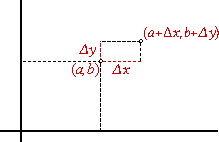
\includegraphics[scale=1.5]{03taylor-dx-dy.pdf}
  \caption{\textbf{$\Delta x$ and $\Delta y$:} Taylor's formula lets us
    approximate a function $z=f(x,y)$ at points $(x,y) = (a+\Delta x, b+\Delta
    y)$ close to $(a,b)$.  The expansion gives us $f(x,y) = f(a+\Delta x,
    b+\Delta y)$ as a function of $\Delta x$ and $\Delta y$.}
\end{figure}
The first three terms are exactly the linear approximation
\eqref{eq:linear-approximation-no-error} of the function that we saw in
Chapter~III, \S~\ref{sec:linear-approximation-no-error}.  The next terms in ~\ref{eq:second-order-taylor} are
\[
\frac{1}{2}f_{xx}(a, b)(\Delta x)^2
+ f_{xy}(a,b)\Delta x \Delta y
+ \frac12 f_{yy}(a,b)(\Delta y)^2.
\]
These terms determine a quadratic form in the variables $\Delta x$ and $\Delta
y$. The quantities $\frac12 f_{xx}(a,b)$, etc.~are the coefficients of the form.


As always, the dots in the expansion \eqref{eq:second-order-taylor} contain the
remainder term.  By carefully including the one-variable Lagrange remainder in
the derivation we can get a formula for the remainder in
\eqref{eq:second-order-taylor}.  We will not do that, but it can be shown that
the remainder is $o\left( (\Delta x)^2 + (\Delta y)^2 \right)$, i.e.\ that it is
small compared to the other terms in the expansion, at least when $\Delta x$ and
$\Delta y$ are small.
% :CONTINUE HERE

\subsection{Example -- compute the Taylor expansion of $f(x, y) = \sin2x\cos y$
  at the point $(\frac16\pi, \frac16\pi)$}
%\marginpar{\dfnt%
%maybe $x^2\ln y	$ is an easier example?}
To find the expansion we need to compute $f, f_x, f_y, f_{xx},
f_{xy},$ and $f_{yy}$ at $(\frac16\pi, \frac16\pi)$.  Here goes:
\[
\begin{aligned}
  f&= \sin 2x \cos y = \tfrac 34 \\
  f_x&=2\cos 2x\cos y = \tfrac12\sqrt{3}\\
  f_y&=-\sin2x \sin y = -\tfrac 14\sqrt3 
\end{aligned}
\qquad
\begin{aligned}
  f_{xx}&=-4\sin2x\cos y = -3 \\
  f_{xy}&=-2\cos 2x\sin y = -\tfrac12 \\
  f_{yy}&=-\sin 2x\cos y = -\tfrac 34.
\end{aligned}
\]
Substituting in the Taylor expansion we get
\begin{align*}
  f\bigl( \tfrac16\pi+\Delta x, &\tfrac16\pi+\Delta y\bigr)\\
  &=
  \tfrac 34 +\tfrac12\sqrt3 \,\Delta x -\tfrac14\sqrt3\,\Delta y
  +\frac12\Bigl\{
  -3(\Delta x)^2 -2\cdot\tfrac12 \Delta x \Delta y - \tfrac34 (\Delta
  y)^2
  \Bigr\} + \cdots\\
  &=\tfrac 34 +\tfrac12\sqrt3 \,\Delta x -\tfrac14\sqrt3\,\Delta y
  -\tfrac32(\Delta x)^2 -\tfrac12 \Delta x \Delta y -\tfrac38(\Delta y)^2
  +\cdots
\end{align*}
Note that the first three terms in the expansion are the linear
approximation of the function:
\[
f\bigl( \tfrac16\pi+\Delta x, \tfrac16\pi+\Delta y\bigr)
= \tfrac 34 +\tfrac12\sqrt3 \, \Delta x -\tfrac14\sqrt3\, \Delta y +\cdots
\]

\subsection{Another example -- the Taylor expansion of $f(x, y) = x^3+y^3-3xy$
  at the point $(1,1)$}
\label{sec:taylor-example-at-minimum}
The function $f(x, y) = x^3+y^3-3xy$ has the
following derivatives at $(1,1)$:
\[
\begin{aligned}
  f & =  x^3+y^3-3xy &= 1 \\
  f_x&= 3x^2 - 3y &= 0 \\
  f_y&= 3y^2-3x &= 0
\end{aligned}\hspace{0.25\textwidth}
\begin{aligned}
  f_{xx} &= 6x &=&\;6 \\ f_{xy} &=-3 &=&-3 \\ f_{yy} &= 6y &=&\;6
\end{aligned}
\]
The first derivatives vanish, so $(1,1)$ is a critical point of $f$.
The second order Taylor expansion of $f$ at $(1,1)$ is
\begin{equation}\label{eq:example-taylor-expansion}
  f(1+\Delta x, 1+\Delta y)
  = 1 + 3(\Delta x)^2 - 3\Delta x \Delta y + 3(\Delta y)^2 +\cdots
\end{equation}
Note that there are not first order terms in this expansion because $(1,1)$ is a critical point -- the coefficients of the first order terms are both zero.

To see what kind of critical point $(1,1)$ is, we have to analyze the second
order, quadratic, terms
\begin{equation}
  3(\Delta x)^2 - 3\Delta x \Delta y + 3(\Delta y)^2.
  \label{eq:example-quadratic-form}
\end{equation}
This expression is a quadratic form in $\Delta x$ and $\Delta y$, and by
completing the square (see Chapter~III, \S~\ref{sec:quadratic-forms}) we
find that
\[
3(\Delta x)^2 - 3\Delta x \Delta y + 3(\Delta y)^2
=3 \Bigl[\bigl(\Delta x - \tfrac 12 \Delta y\bigr)^2
  + \tfrac 34 (\Delta y)^2\Bigr].
\]
In particular, the quadratic terms in the Taylor expansion of $f$ at the
critical point are always positive, no matter what $\Delta x$ and $\Delta
y$ we choose (as long as they are not both zero).  If we are allowed to
ignore the remainder term (the ``$\cdots$''), then this implies that the
function has a local minimum: after all, the Taylor expansion
(\ref{eq:example-taylor-expansion}) says that for small $\Delta x$ and
$\Delta y$ the function value $f(1+\Delta x, 1+\Delta y)$ is 
\[
f(1+\Delta x, 1+\Delta y) \approx 
f(1, 1) + 3 \bigl(\Delta x - \tfrac 12 \Delta y\bigr)^2
  + \tfrac 94 (\Delta y)^2. 
\]
The second order terms are all positive, so the Taylor expansion tells us that
\[
f(1+\Delta x, 1+\Delta y) \geq f(1,1),
\]
at least for small $\Delta x$ and $\Delta y$.  The function therefore has a local minimum at $(1,1)$.

\subsection{Example of a saddle point}
\label{sec:taylor-example-at-saddle}
The same function $f(x,y) = x^3+y^3-3xy$ has another critical point,
namely, the origin.  By calculating the derivatives at $(0,0)$ we
find that the Taylor expansion at the origin is
\begin{equation}\label{eq:example-taylor-at-origin}
  f(\Delta x, \Delta y) = -3\Delta x \Delta y + \cdots
\end{equation}
Ignoring the remainder terms we see that near the origin $f(\Delta x,
\Delta y) \approx -3\Delta x \Delta y$, which suggests that $f$ is
negative when $\Delta x$ and $\Delta y$ are both positive, or when
they are both negative, while $f$ is positive when $\Delta x$ and
$\Delta y$ have opposite signs.

Arbitrarily close to the origin the function $f$ therefore has both
positive and negative values, and therefore $f$ has neither a local
maximum nor a local minimum at the origin.  In fact the Taylor
expansion (\ref{eq:example-taylor-at-origin}) suggests that the graph
of $f$ should look like that of the ``saddle function'' $z=xy$.

\subsection{The two-variable second derivative test}   
The last two examples essentially show us how the second derivative test
for functions of two variables works.  To explain how it works in general,
let's suppose a function $f$ has a critical point at $(a,b)$.  Then the
first partial derivatives of $f$ vanish at $(a,b)$ and hence the Taylor
expansion has no first order terms.  We get
\begin{multline}\label{eq:two-variable-expansion-at-cpt}
  f(a+\Delta x, b+\Delta y) 
  = f(a, b) +\\
  \frac{1}{2}\Bigl\{
  f_{xx}(a, b)(\Delta x)^2 + 2f_{xy}(a,b)\Delta x \Delta y +
  f_{yy}(a,b)(\Delta y)^2
  \Bigr\} +\cdots
\end{multline}
This is the two-variable analog of equation
\eqref{eq:one-variable-expansion-at-cpt}.  To see if $(a, b)$ is a local maximum or minimum (or something else), we have to see if the quadratic terms in \eqref{eq:two-variable-expansion-at-cpt} are always negative, always positive, or if they can have either sign, depending on the choice of $\Delta x$, $\Delta y$.

The precise statement of the second derivative test uses the
terminology introduced in Chapter~I, \S\ref{sec:quadratic-forms} and Figure~\ref{fig:typical-q-forms} in that chapter.

\subsection*{Theorem (second derivative test)}\itshape  
If $(a, b)$ is a critical point of $f(x, y)$, and if 
\[
Q(\Delta x, \Delta y) = 
  \frac{1}{2}\Bigl\{
  f_{xx}(a, b)(\Delta x)^2 + 2f_{xy}(a,b)\Delta x \Delta y +
  f_{yy}(a,b)(\Delta y)^2
  \Bigr\}
\]
is the quadratic part of the Taylor expansion of $f$ at the critical
point, then 
\begin{itemize}
\item[$\blacktriangleright$] If $Q$ is \textbf{positive definite} then
  $(a,b)$ is a \textbf{local minimum} of $f$,
\item[$\blacktriangleright$] If $Q$ is \textbf{negative definite} then
  $(a,b)$ is a \textbf{local maximum} of $f$,
\item[$\blacktriangleright$] If $Q$ is \textbf{indefinite} then $(a,
  b)$ is a \textbf{saddle point} of $f$
\item[$\blacktriangleright$] If $Q$ is \textbf{semidefinite} the second
  derivative test is inconclusive.
\end{itemize}
\upshape
When the form $Q$ is indefinite, so that it can be factored as
\[
Q(\Delta x, \Delta y) = (k\Delta x + l\Delta y)(m\Delta x+n\Delta y),
\]
then the level set of the function $f$ containing the critical point
$(a, b)$ consists of two curves. One of these curves is tangent to the
line
\[
k\Delta x+l\Delta y = 0, \text{ i.e. } k(x-a) + l(y-b) = 0
\]
while the other is tangent to
\[
m\Delta x+n\Delta y = 0, \text{ i.e. } m(x-a) + l(y-b) = 0.
\]

\subsection{Example -- apply the second derivative test to the fishy example}
In \S~\ref{sec:cubic-maxmin-exist} and \S~\ref{sec:critical-fish} we had
found that the function $f(x, y) = x^2-x^3-y^2$ has two critical points,
one at the origin, and one at the point $(\frac 23, 0)$.
\begin{figure}[h]
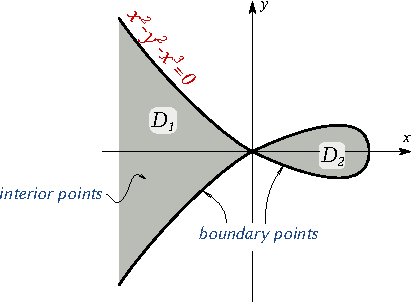
\includegraphics[width=0.5\textwidth]{03maxminexistence.pdf}
\end{figure}
By carefully
looking at the zero set of the function we discovered that the origin is
neither a local maximum nor a local minimum, and that the point $(\frac 23,
0)$ is a local maximum.  The second derivative test provides a more
systematic way of reaching these conclusions.  To apply the test we need to
know the second derivatives of $f$ at the critical points.  They are:
\begin{center}
  \begin{tabular}{cccc}\hline
    \rule[-6pt]{0pt}{16pt}
    $(x, y)$  &$f_{xx}(x, y)$ &$f_{xy}(x, y)$ &$f_{yy}(x, y)$ \\\hline
    \rule[-4pt]{0pt}{16pt}
    $(x, y)$ & $ 2-6x $  & $0$  &  $-2$ \\
    \rule[-4pt]{0pt}{14pt}
    $(0,0)$ & $2$ & $0$ & $-2$ \\
    \rule[-6pt]{0pt}{16pt}
    $(\tfrac23, 0)$ & $-2$ & $0$ &$-2$\\\hline
  \end{tabular}
\end{center}

Therefore the second order Taylor expansion of $f$ at the origin is
\begin{align*}
  f(\Delta x, \Delta y)
  &= f(0,0) + \tfrac12 \bigl\{ 2\cdot (\Delta x)^2 +
  2\cdot 0\cdot \Delta x \Delta y + (-2) (\Delta y)^2 \bigr\} +\cdots\\
  &=  (\Delta x)^2 - (\Delta y)^2 + \cdots\\
  &=  (\Delta x - \Delta y)(\Delta x+\Delta y) + \cdots\\
\end{align*}
The quadratic part of the Taylor expansion can be factored, so this is the ``indefinite'' case.  It can be both positive and negative, depending on our choice of $\Delta x$ and $\Delta y$.  The second derivative test implies that the origin is a saddle point. It also says that the zero set of $f$ near the origin consists of two curves, whose tangents at the origin are given by the two equations
\begin{equation}
\Delta x-\Delta y =0 \text{ and } \Delta x+\Delta y = 0.
\label{eq:second-deriv-test-fishy-at-origin}
\end{equation} 
In this case the point $(a, b)$ is the origin, so $\Delta x = x-a = x$
and $\Delta y = y-b = y$, and the two tangents are the lines $y=\pm
x$.

The second order Taylor expansion at the other critical point $(\frac 23, 0)$ is given by
\begin{equation}
f(\tfrac23 + \Delta x, \Delta y)
= f(\tfrac23, 0) - (\Delta x)^2 - (\Delta y)^2 + \cdots
\label{eq:second-deriv-test-fishy-at-eye}
\end{equation}
This time we see that the second order terms of the Taylor expansion are negative definite. The second derivative test therefore says that we have a local maximum at $(\frac 23, 0)$.




\section{Problems}  
\begin{multicols}{2}
\problemfont
\problem [for discussion] Are $\Delta x$ in \S~\ref{sec:taylor-example-at-minimum}
and \S~\ref{sec:taylor-example-at-saddle} the same?

Are the $\Delta x$ in the equations \eqref{eq:second-deriv-test-fishy-at-origin} and
in \eqref{eq:second-deriv-test-fishy-at-eye} of the second derivative test example
the same?  Explain what they stand for.
\answer
The two $\Delta x$ and $\Delta y$'s are different.  The first set of $(\Delta
x,\Delta y)$ are 
\[
  \Delta x = x-0, \qquad \Delta y = y-0,
\]
$(0,0)$ being the coordinates of the first critical point we studied.  The second set
of $(\Delta x,\Delta y)$ is
\[
  \Delta x = x-\tfrac23, \qquad \Delta y = y-0,
\]
where $(\frac23, 0)$ is the other critical point.  In a drawing:
\begin{figure}[h]
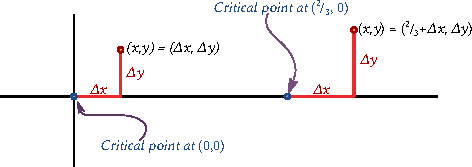
\includegraphics{answer-whichDxDy.pdf}
\end{figure}
\endanswer

\problem
Compute the second order Taylor expansion of the following functions
at the indicated points:

[In this problem you are asked to find Taylor expansions of functions
at various points.  Since these points are not necessarily critical points, the
expansions you find will generally have first and second oder terms.
In the expansions you will compute when you use the second derivative
test later on, there will be no first order terms.]

\subprob $f(x, y) =\bigl(1-x+xy\bigr)^2$ at $(0,0)$
\answer 
$f(\Delta x, \Delta y)
= \Bigl(1-\Delta x+\Delta x\Delta y\Bigr)^2
= 1-2\Delta x+\Delta x^2+2\Delta x\Delta
y+\cdots$
\endanswer

\subprob  $f(x, y) =\bigl(1-x+xy\bigr)^2$ at $(1,1)$ 
\answer
$f(1+\Delta x, 1+\Delta y)
= \Bigl(1-(1+\Delta x)+(1+\Delta x)(1+\Delta y)\Bigr)^2
=
1+2\Delta y+2\Delta x\Delta y+2(\Delta y)^2+\cdots$
\endanswer

\subprob  $f(x, y) =e^{x-y^2}$ at $(0,0)$ 
\answer
$f(\Delta x,\Delta y) = e^{\Delta x-(\Delta y)^2} =
1+\Delta x+\frac{1}{2}(\Delta x)^2 -(\Delta y)^2+\cdots$
\endanswer

\subprob  $f(x, y) =e^{x-y^2}$ at $(1,1)$
\answer
$f(1+\Delta x, 1+\Delta y)
= e^{(1+\Delta x)-(1+\Delta y)^2}
=
1+\Delta x - 2\Delta y+ \frac{1}{2}(\Delta x)^2 - 2\Delta x\Delta y
+(\Delta y)^2+\cdots$
\endanswer

\subprob  $f(x, y) =\dfrac{x}{1-y}$ at $(0,0)$ 

\subprob  $f(x, y) =\dfrac{x}{1+y}$ at $(1,0)$ 

\problem Factor, or complete the square in the following quadratic 
forms, draw their zero sets, and determine if they are positive
definite, negative definite, indefinite or degenerate.

\subprob $Q(x, y) = x^2+3xy+y^2$ 

\subprob $Q(x, y) = x^2 + xy + y^2$  

\subprob $Q(x, y) = 2x^2 +3xy - 4y^2$  

\subprob $Q(x, y) = 2x^2 + 3xy - 5y^2$ 

\subprob $Q(\Delta x, \Delta y) = (\Delta x)^2 + (\Delta y)^2$  

\subprob $Q(\Delta x, \Delta y) = (\Delta x)^2 - 3(\Delta y)^2$  

\subprob $Q(\Delta x, \Delta y) = \Delta x \Delta y$ 

\subprob $Q(\Delta x, \Delta y) = \Delta x \Delta y -2 (\Delta y)^2$ 

\problem If $a$ is a constant, then for which values 
of $a$ is the form $Q(x, y) = x^2 + 2axy + y^2$ positive/negative
definite, indefinite, or degenerate?
\answer  Complete the square and you get
\[
Q(x, y) = \bigl(x-ay\bigr)^2 + \bigl(1- a^2\bigr)y^2. 
\]
When $1-a^2>0$, i.e.\ when $-1<a<1$ the form is positive definite.
When $a=\pm 1$ the form is a perfect square, namely, 
\[
x^2 \pm 2xy + y^2 = \bigl(x\pm y\bigr)^2.
\]
When $1-a^2<0$, i.e.\ when $a>1$ or $a<-1$, the form is indefinite:
\[
x^2 + 2axy + y^2 = 
\Bigl(x-ay-\sqrt{a^2-1}y\Bigr)
\Bigl(x-ay+\sqrt{a^2-1}y\Bigr)
=(x-k_+y)(x-k_-y),
\]
where $k_\pm = -a \pm \sqrt{a^2-1}$.

\endanswer

\problem \label{prb:lots-of-2nd-deriv-tests} 
Find all critical points of the following functions (you did many of
these in problem \ref{prb:find-critical-points}).  Apply the second
derivative test to all critical points you find.
\answer 
See the solutions to Problem \ref{prb:find-critical-points} for the
solutions to this problem.
\endanswer

\subprob\hbox to0.45\textwidth{$f(x,y)=x^2+4y^2-2x+8y-1$\hfill} 

\subprob $f(x,y)=x^2-y^2+6x-10y+2$ 

\subprob $f(x,y)=x^2+4xy+y^2-6y+1$ 

\subprob $f(x,y)=x^2-xy+2y^2-5x+6y-9$ 

\subprob $f(x,y)=y^2-18 x^2+x^4$ 

\subprob $f(x,y)=y^4-4y^2-18 x^2+x^4$ 

\subprob $f(x,y)=9+4x-y-2x^2-3y^2$ 

\subprob $f(x,y)=xy(4-x-2y)$ 

\subprob $f(x,y)=x(x-y)(x-1)$ 

\subprob $f(x,y)=(x-y)(xy-4)$ 

\subprob $f(x,y)=y^2+\cos x$ 

\subprob $f(x,y)=x^2y-\frac13 y^3$ 

\subprob $f(x,y)=(x-y^2)(x-1)$ 

\subprob $f(x,y)=(x-y)(xy-4)$ 

\subprob $f(x,y)=x^2$ 

\subprob $f(x,y)=x^2-y^4$ 

\subprob $f(x,y)=x^2+y^4$ 

\subprob $f(x,y)=x^2y$ 


\problem % about f(x, y) = sin x sin y  
\subprob Draw the zero set of the 
function $f(x, y) = \sin(x) \sin(y)$.
\subprob Where is the function $f$ positive? 
Find as many critical points as you can without computing $f_x$ or
$f_y$.

\subprob Find all critical points of $f(x, y)$.  
Which are local minima or local maxima?


\problem Find all critical points of the following functions, and
apply the second derivative test to the points you find.

\subprob 
$f(x, y) = x^2 + y^2 - \tfrac12 xy^2$
\answer 
$f_x = 2x-\frac12y^2$, $f_y = 2y-xy$.  
The equation $f_y=y(2-x)=0$ leads to two possibilities: $x=2$ or
$y=0$.  If $y=0$ then $f_x=0$ implies $x=0$, which gives us one
critical point, the origin $(0,0)$.  If on the other hand $x=2$, then
$f_x=0$ implies $y^2=8 \iff y=\pm2\sqrt{2}$.  We therefore get two
more critical points $(2, \pm 2\sqrt{2})$.

The second derivatives are $f_{xx} = 2$, $f_{xy} = -y$, $f_{yy} =
2-x$.  Therefore we have the following Taylor expansions at the
three critical points:
\begin{align*}
    f(\Delta x, \Delta y) 
    &= f(0,0) + (\Delta x)^2 + (\Delta y)^2 + \cdots
    &\implies \text{loc.min.}\\
    f(2+\Delta x, 2\sqrt{2} + \Delta y) 
    &= f(2, 2\sqrt{2}) + (\Delta x)^2 - 2\sqrt{2} \Delta x \Delta y +
    0(\Delta y)^2+\cdots\\
    &= f(2, 2\sqrt{2}) + \bigl(\Delta x - 2\sqrt{2} \Delta y\bigr)
    \Delta x +\cdots
    &\implies \text{saddle}\\
    f(2+\Delta x, -2\sqrt{2} + \Delta y) 
    &= f(2, -2\sqrt{2}) + (\Delta x)^2 + 2\sqrt{2} \Delta x \Delta y +
    0(\Delta y)^2+\cdots\\
    &= f(2, -2\sqrt{2}) + \bigl(\Delta x + 2\sqrt{2} \Delta y\bigr)
    \Delta x +\cdots
    &\implies \text{saddle}
\end{align*}
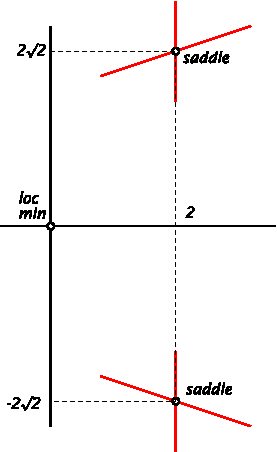
\includegraphics[width=96pt]{03answers005.pdf}
The origin is therefore a local minimum, and the points $(2,
\pm2\sqrt{2})$ are saddle points.  At $(0, 2\sqrt{2})$ the level set
consists of two crossing curves, whose tangents are given by
$\Delta x=0$ (a vertical line) and $\Delta x=2\sqrt{2}\Delta y$ (a line
with slope $1/2\sqrt{2} = \frac14\sqrt{2}$).
\endanswer

\subprob $f(x, y) = x^2 + y^2 - x^2y^2$ 

\subprob $f(x,y) = x+2y - xy^2$ 
\answer 
$f_x = 1-y^2$, $f_y = 2-2xy$.  
Critical points: $f_x=0$ holds when $y=\pm 1$.  If $y=+1$, then
$f_y=0$ implies $x=1$, and if $y=-1$ then $f_y=0$ implies $x=-1$.
There are therefore two critical points, $(1,1)$ and $(-1,-1)$.
\endanswer

\subprob $f(x, y) = 8x^4 + y^4 - xy^2$ 

\problem Suppose that $f(x,y)=x^2+y^2+kxy$. Find and classify the critical  
points, and discuss how they change when $k$ takes on different values.

\problem Consider the function
\[
f(x,y)=x^3-3xy^2.
\]
The graph of this function is known as the ``Monkey Saddle.''

\subprob Show that $(0,0)$ is the only critical point of $f$. 

\subprob Show that the second derivative test is inconclusive for $f$. 

\subprob Draw the zero set of $f$, and indicate where $f>0$ and where $f<0$. 

\subprob What kind of critical point is $(0,0)$? 

\problem Consider the function
\[
f(x,y)=x^3 - x^2y.
\]
\subprob Draw the zeroset of $f$ and indicate where $f(x,y)$ is positive, and where
$f(x,y)$ is negative.

\subprob Find all the critical points of the function.  

\subprob Does the second derivative test apply to any of the critical points of
$f$?

\subprob Use the sign-diagram you made in part \textbf{(a)} to decide which critical
points are local maxima or minima.
\noproblemfont
\end{multicols}

\section{Second derivative test for more than two variables}
The ideas that lead to the second derivative test for functions of two variables
also work when we have a function with more variables.  However, the second
derivative test for functions of more than two variables is beyond the scope of
Math~234, and this short section tries to explain why.

\subsection{The second order Taylor expansion}   
If $z=f(x_1, x_2, \cdots, x_n)$ is a function of $n$ variables, then its Taylor
expansion of order two at some point $(a_1, a_2, \cdots, a_n)$ turns out to be
\begin{align*}
  f(a_1+\Delta x_1, \cdots, a_n&+\Delta x_n) = \\
  f(a_1, \cdots, a_n) + &f_{x_1} \Delta x_1 + \cdots + f_{x_n} \Delta  x_n + \\
  &\begin{aligned} \frac12\Bigl\{ &f_{x_1x_1} (\Delta x_1)^2 + \cdots +
    f_{x_1x_n}\Delta x_1\Delta x_n \\
    +&f_{x_2x_1}\Delta x_2\Delta x_1 +\cdots + f_{x_2x_n}\Delta x_2\Delta x_n \\
    &\hspace{8em}\vdots\\
    +&f_{x_nx_1}\Delta x_n\Delta x_1 +\cdots + f_{x_nx_n}(\Delta x_n)^2 \Bigr\}
    + \cdots
  \end{aligned}
  \label{eq:03n-variable-Taylor}
\end{align*}
where the partial derivatives $f_{x_i}$ and $f_{x_ix_j}$ are to be evaluated at
the point $(a_1, \cdots, a_n)$.  The same trick involving the function
``$g(t)$'' that was used in \S\ref{sec:Taylor-derived} to derive the
two-variable Taylor expansion works without modification.

If $(a_1, \cdots, a_n)$ is a critical point then $f_{x_1} = f_{x_2} = \cdots =
f_{x_n} = 0$, so the linear terms are absent, and the function is described by
the quadratic terms of the Taylor expansion
\begin{align*}
  f(a_1+\Delta x_1, \cdots, a_n+\Delta x_n)& = \\
  f(a_1, \cdots, a_n) +\frac12\Bigl\{
  &f_{x_1x_1} (\Delta x_1)^2 + \cdots + f_{x_1x_n}\Delta x_1\Delta x_n \\
  +&f_{x_2x_1}\Delta x_2\Delta x_1 +\cdots + f_{x_2x_n}\Delta x_2\Delta x_n \\
  &\hspace{8em}\vdots\\
  +&f_{x_nx_1}\Delta x_n\Delta x_1 +\cdots + f_{x_nx_n}(\Delta x_n)^2 \Bigr\} +
  \cdots
\end{align*}
Just as in the two-variable case we could now try to see if the quadratic terms
are positive definite or negative definite by completing squares.  The procedure
is however much more complicated, and best understood in terms of
\textit{``eigenvalues of matrices,''} a subject which is explained in courses on
linear algebra or matrix algebra (Math~320, 340, or 341).  Therefore, we will
only use the second derivative test for functions of two variables in this
course.


\section{Optimization with constraints and the method of Lagrange multipliers}
In many optimization problems we want to find the maximal or minimal value of a
function $f(x, y)$ where $(x, y)$ can be any point satisfying a certain
\emph{constraint}
\begin{equation}
  g(x, y) = C.
  \label{eq:03the-constraint}
\end{equation}
Thus the domain $D$ of the function we want to minimize consists of all points $(x,
y)$ that satisfy the equation $g(x,y) = C$: it is a level set of $g$.

\subsection{Solution by elimination or parametrization}
One approach to minimization problems with a constraint is to ``eliminate one
variable.''  If we are asked to find the minimal value that $f(x,y)$ can have if
$(x, y)$ must satisfy the constraint $g(x, y)=C$, then we first try to solve the
constraint equation for one of the variables, say, for $y$:
\[
g(x, y) = C \iff y=h(x).
\]
Now the only $(x, y)$ that we have to consider are points of the form $(x, h(x))$,
so the old minimization problem is equivalent to a new problem: find the minimal
value of $F(x) = f(x, h(x))$, where there are no constraints on $x$.  This new
problem is a one variable problem of the kind we learned to solve in Math~221.

\subsection{Example -- which rectangle with perimeter 1 has the largest area?}
\label{sec:isoperimetric-1}
This is another problem, like finding the tangent to the parabola $y=x^2$, that
appears in almost every first semester calculus course.  We recall its solution.

If the sides of the rectangle are $x$ and $y$, then its area is $xy$ and its
perimeter is $2(x+y)$.  Hence the function we want to maximize is $f(x, y) = xy$ and
the constraint is
\[
g(x, y) = 2(x+y) = 1.
\]
\marginpar{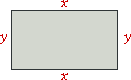
\includegraphics{03rectangle.pdf}}%
Solving the constraint for $y$ tells you that $y= \frac12-x$, so we want to maximize
the function $F(x) = f(x, \frac12 - x) = x(\frac12 - x)$.  The only remaining
constraint is that $x$ cannot be negative, and that $y=\frac12-x$ also cannot be
negative.  Thus we want to maximize $F(x) = x(\frac12-x)$ over all $x$ in the
interval $0\leq x\leq\frac12$.

\subsection{Example -- maximize $x+2y$ over the unit circle}

We are asked to find the maximal value of $f(x, y) = x+2y$ where $(x,y)$ is allowed
to be any point that satisfies the constraint $g(x, y) = x^2 + y^2 = 1$.  If we try
to solve for $y$ we find that there are two solutions, $y=\pm\sqrt{1-x^2}$, and so
the ``function'' $F(x) = x+2y = x\pm 2\sqrt{1-x^2}$ is not really a function at all.
In this case we can still solve the problem by noting that any point on the unit
circle can be written as $(x,y) = (\cos \theta, \sin \theta)$ for some angle
$\theta$, and thus we have to maximize the function
\[
F(\theta) = f(\cos \theta, \sin \theta) = \cos \theta + 2\sin \theta.
\]
Here there are no constraints on $\theta$, and we again have a first semester
calculus problem.


\subsection{Solution by Lagrange multipliers} 
In both examples above we were lucky because we could either solve the constraint
equation or we could parametrize all possible points that satisfy the constraint.
There is a method due to Joseph-Louis Lagrange (known from the remainder term) that
does not require this kind of luck.  His method is based on the following observation
(see Figure~\ref{fig:03lagrangemultipliers}).
\begin{figure}[hb]
  \begin{center}
    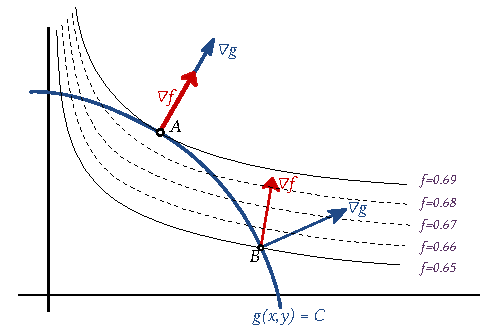
\includegraphics{03lagrangemultipliers.pdf}
  \end{center}
  \caption{Lagrange multipliers: if, at some point like $B$ on the constraint set the
    gradients of $f$ and $g$ are not parallel, then we can increase $f$ by moving
    along the constraint set in the direction of $\nab f$.  At a point (such as $A$)
    where the function $f$ reaches a maximum, the gradients $\nab f$ and $\nab g$
    must be parallel.}
  \label{fig:03lagrangemultipliers}
\end{figure}

Let $B=(x, y)$ be a point on the constraint set as in the figure.  Assume that $\nab
g\neq\vvv0$ at $B$, then near $B$ the Implicit Function Theorem says that the
constraint set $g(x, y) = C$ is a curve, and that its tangent is perpendicular to
$\nab g(B)$.

If $\nab f(B)$ is not perpendicular to the constraint set at $B$, then it provides us
a direction along the constraint set in which $f$ will increase (see
Figure~\ref{fig:03lagrangemultipliers}).  Therefore $f$ does not have a maximum at
$B$.  It follows that at a maximum of $f$ on the constraint set $g(x, y)=C$ the
gradient $\nab f(B)$ must be perpendicular to the constraint set, and hence it must
be parallel to $\nab g(B)$.  Since one vector is parallel to another if it is a
multiple of the other vector, we have found the following fact.

\subsection{Theorem (Lagrange multipliers)}  
\itshape If the function $z=f(x, y)$ attains its largest value among all points that
satisfy the constraint $g(x, y) = C$ at the point $(a, b)$, and if
\begin{equation}
  \nab g(a,b) \neq 0 ,
\end{equation}
then the point $(a, b)$ satisfies the \textit{Lagrange Multiplier} equation,
\begin{equation}
  \nab f(a, b) = \lambda \nab g(a, b)
  \label{eq:Lagrange-multiplier} 
\end{equation}
\upshape The number $\lambda$ is called the \textit{Lagrange multiplier}, and it is
one of the unknowns in the equations we must solve when we use Lagrange's method.

\subsection{Example} We again try to find the largest rectangle with
perimeter~$1$, as in example \ref{sec:isoperimetric-1}.

The problem is to maximize $f(x, y) = xy$ with constraint $g(x, y) = 2x+2y = 1$.  We
compute the gradients
\[
\nab f = \vek y \\ x\tor, \qquad \nab g = \vek2\\2\tor,
\]
The gradient of $g$ never vanishes, i.e.\ $\nab g(x,y)\neq\vvv0$ for all $(x, y)$, so
Lagrange tells us that at any minimum or maximum the following equations hold:
\begin{align*}
  f_x = \lambda g_x, &\text{ i.e. } y=2\lambda \\
  f_y = \lambda g_y, &\text{ i.e. } x=2\lambda \\
  g(x, y)=C, &\text{ i.e. } 2x+2y=1.
\end{align*}
The first two equations come from $\nab f = \lambda \nab g$, and the last equation is
the constraint.  We have three equations, and we also have three unknowns: $x$, $y$
and the Lagrange multiplier $\lambda$.

In this case it is easy to solve the equations: the first two say that both $y$ and
$x$ equal $2\lambda$, so in particular, they equal each other: $y=x$.  This already
tells us that the solution is a square!  To complete the problem we must still solve
for $x, y, \lambda$. Since $x=y$ the constraint implies $4x=1$, so $x=y=\frac14$.
Finally, either of the first two equations provides $\lambda = \frac12x =\frac12y =
\frac18$.

\subsubsection*{What is the meaning of $\lambda$?}  In this example you
see that we first found the solution $(x, y)$, and then computed
$\lambda$.  The multiplier $\lambda$ is the ratio between the lengths of
the gradients of $f$ and $g$ at the maximum, and can be interpreted as
\textit{the rate at which the maximum $f$ changes if the value of the
constraint $g=C$ is varied};  the details go beyond this course (but see
Problems~\ref{prb:lagrange-multiplier-interpretation-1} and
\ref{prb:lagrange-multiplier-interpretation-2}).  In any case, the
upshot is that, when using Lagrange's method, \textit{you must always
also find $\lambda$,} or at least make sure that a $\lambda$ exists for
the $x$ and $y$ you have found.


\subsubsection*{Did we find a maximum or a minimum?}  Lagrange's method does not tell us if
we have a maximum or a minimum, and we will have to use different methods to figure
this out.  There does exist a second derivative test for constrained minimization
problems, but it falls outside the scope of this course.

\subsection{A three variable example}  
\textit{Find the largest value of $x+y+z$ on the sphere with equation $x^2 + y^2 +
  z^2 = 1$.}

\textit{Solution: } We must maximize $f(x, y, z) = x+y+z$ with constraint $g(x, y,
z)= x^2 + y^2 + z^2 = 1$.

Lagrange's method says that the minimum and maximum either occur at a point $(x_0,
y_0, z_0)$ with $\nab g(x_0, y_0, z_0) = \vvv0$, or else at a point that satisfies
Lagrange's equations.  The gradient of $g$ is
\[
\nab g(x, y, z) = \vek 2x\\2y\\2z\tor,
\]
and the only point where $\nab g = \vvv0$ is at the origin.  The origin does not
satisfy the constraint $g(x, y, z) = 1$, so we can rule out the possibility of the
maximum or minimum occurring at a point with $\nab g=\vvv 0$.

This leads us to consider the Lagrange multiplier equations, which are
\begin{align*}
  1& = \lambda\cdot 2x &(f_x=\lambda g_x)\\
  1& = \lambda\cdot 2y&(f_y=\lambda g_y)\\
  1& = \lambda\cdot 2z&(f_z=\lambda g_z)\\
  x^2 + y^2 + z^2&=1&(g(x, y, z) = C)
\end{align*}
Solve the first three equations for $x, y, z$ and substitute the result in the
constraint, and we find
\[
\frac{1}{4\lambda^2} + \frac{1}{4\lambda^2} + \frac{1}{4\lambda^2} =1 \implies
\frac{3}{4\lambda^2}=1 \implies \lambda = \pm\tfrac12\sqrt{3}.
\]
We therefore find two points on the sphere,
\[
(x, y, z) = \bigl(\tfrac13\sqrt{3}, \tfrac13\sqrt{3}, \tfrac13\sqrt{3} \bigr) \text{
  and } (x, y, z) = \bigl(-\tfrac13\sqrt{3}, -\tfrac13\sqrt{3}, -\tfrac13\sqrt{3}
\bigr)
\]
By computing the function values we find that the first point maximizes $x+y+z$, and
the second minimizes $x+y+z$.

\section{Problems}\problemfont    
\begin{multicols}{2}
\problem Minimize $xy$ subject to the constraint 
\[
x^2+\tfrac14 y^2 = 1.
\]
Draw the constraint set.
\answer 
$f(x, y) = xy$, $g(x, y) = x^2 + \frac14 y^2$. 
$\nab f = \tvek y \\ x\ttor$, $\nab g = \tvek 2x\\ y/2\ttor$.

First we check for possible max/minima which satisfy $\nab g=\vvv0$.
But the only point $(x,y)$ satisfying $\nab g(x,y) = \tvek0\\0\ttor$
is the origin $(x, y) = (0,0)$, and this point does not lie on the
constraint set.

Therefore, \textbf{if} there is a minimum it is attained at a solution
of Lagrange's equations
\begin{align*}
  f_x = \lambda g_x &\iff y = 2\lambda x \\
  f_y = \lambda g_y &\iff x = \lambda y/2 \\
  g(x, y) = 1 & \iff x^2+\tfrac14 y^2 = 1
\end{align*}
Multiply the first equation with $y$ and the second with $4x$, then
you get
\[
y^2 = 2\lambda xy \text{ and } 4x^2 = 2\lambda xy
\]
Hence $y^2 = 4x^2$.  Put that in the constraint, and you find 
\[
1=x^2 + \tfrac14 y^2 = 2 x^2.
\]
Thus $x= \pm\sqrt{1/2} = \pm \frac12 \sqrt{2}$ and $y = \pm \sqrt2$.
In all we have found \emph{four} possible solutions.
Lagrange's method does not tell us which, if any, of these are minima.
\marginpar{\footnotesize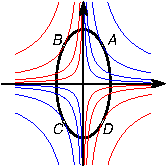
\includegraphics{03answers006.pdf}\\
Level sets of the function $f(x, y) = xy$ and the constraint set
$x^2+\frac14y^2=1$}

By looking at the constraint set (it's an ellipse with horizontal axis
of length 1 and vertical axis of length 2) and taking into account
that $f(x, y) =xy$ is positive in the first and third quadrants, and
negative in the second and fourth, you find out that the two points
$(\frac12\sqrt{2},\sqrt{2})$ and $(-\frac12\sqrt{2},-\sqrt{2})$  ($A$
and $C$ in the figure) are maximum points, while
$(-\frac12\sqrt{2},\sqrt{2})$ and $(\frac12\sqrt{2},-\sqrt{2})$  ($B$
and $D$ in the figure) are minimum points.
\endanswer
\problem A six-sided rectangular box is to hold $1/2$ cubic meter.  Which  
shape should the box be to minimize surface area?

\subprob Find the solution without using Lagrange's method. 
\answer  
Let the sides of the box be $x,y,z$.  We want to minimize the quantity $A =
2xy+2yz+2xz$, with the constraint $V=xyz=\frac12$.  The constraint implies that
$x\neq0$, $y\neq0$ and $z\neq0$ moreover, given $x$ and $y$ the only $z$
which satisfies the constraint is $z=1/(2xy)$.  Thus we must minimize the
following function of two variables
\[
A(x,y) = xy + \frac{1} {2x} + \frac{1} {2y}
\]
over all $x>0$, $y>0$.

A minimum must be an interior minimum (can't be on the $x$ or $y$-axis
since these are excluded), and thus must be a critical point.
\[
\pdd Ax = y-\frac{1} {2x^2}, \qquad
\pdd Ay = x - \frac{1} {2y^2}.
\]
Solving $A_x=A_y=0$ for $(x,y)$ leads to $x=y=\sqrt[3]2$, so the solution
is a cube $1/\sqrt[3]{2}$ on a side
\endanswer

\subprob Use Lagrange multipliers to solve this problem. 
\answer 
We wish to minimize $A(x,y,z) = 2yz+2xz+2xy$ with constraint
$V(x, y, z) = xyz = \frac12$, using Lagrange's method.

First we check for exceptional points on the constraint set, i.e.\
points $(x,y,z)$ that satisfy both $V(x, y, z) = \frac12 $ and
$\nab V(x, y, z) = \vvv0$.  Since 
\[
\nab V = \vek yz \\ xz\\ xy\tor
\]
the gradient $\nab V$ vanishes if at least two of the three
coordinates $x, y, z$ are zero.  But such a point can never satisfy
the constraint $xyz=\tfrac12$.  Therefore, if there is a box with
least area, its sides $x, y, z$ must satisfy Lagrange's equations.

Lagrange's equations are
\begin{align*}
  A_x = \lambda V_x &\iff 2y+2z = \lambda yz\\
  A_y = \lambda V_y &\iff 2x+2z = \lambda xz\\
  A_z = \lambda V_z &\iff 2x+2y = \lambda xy
\end{align*}
To get rid of $\lambda$ multiply the first equation with $x$ and the
second with $y$ to get
\[
y(2x+2z) = \lambda xyz = x(2y+2z) \implies
2xy+2yz = 2xy+2xz \implies 2yz=2xz.
\]
Therefore we find that either $z=0$ or $x=y$.  
But $z=0$ is not possible, because $(x,y,z)$ must satisfy the
constraint $xyz=0$.  Therefore we get $x=y$.

If you multiply the second Lagrange equation with $y$ and the third
with $z$ then the same reasoning as above tells you that $y=z$.

So, \emph{if there is a minimum} then it happens when $x=y=z$, i.e.\
when the box is a cube.  The only cube that satisfies the constraint
has sides $x=y=z=2^{-1/3}$.

As always, Lagrange's method does not rule out the possibility that
the cube we have found actually maximizes the surface area, rather
than minimizing it.  That this is actually not the case is something
you would have to prove by other means.  We will not do that in this
course.

\endanswer
\problem Using the methods of this section, find the shortest distance from  
the origin to the plane $x+y+z=10$.  (suggestion: instead of
minimizing the distance, you can also minimize the square of the
distance.)
\answer  Answer: the shortest distance is $\sqrt{100/3}$.  

Solution:  If $(x, y, z)$ is any point than its distance to the origin
is $d(x, y, z) = \sqrt{x^2+y^2+z^2}$.  We want to minimize $d(x, y,
z)$ over all points $(x, y, z)$ which satisfy the constraint
$g(x, y, z) = x+y+z=10$.  Instead of minimizing $d(x, y, z)$ we will
minimize $f(x, y, z) = d(x, y, z)^2 = x^2+y^2+z^2$.  You can do this
problem directly with the function $d(x,y,z)$ and you will get the
same answer -- the computations are just a little longer because
$f$ has easier derivatives than $d$.

We use Lagrange's method.  First we check for exceptional points,
i.e.\ points on the constraint set which satisfy $\nab g=\vvv0$.
Since $\nab g = \tvek1\\1\\1\ttor$ the gradient of $g$ can never be
the zero vector, so there are no exceptional points.  If there is a
minimum of $f$ on the constraint set, it must be a solution of
Lagrange's equations.

The Lagrange equations are 
\begin{align*}
  f_x=\lambda g_x &\iff 2x = \lambda\\
  f_y=\lambda g_y &\iff 2y=\lambda\\
  f_z=\lambda g_z &\iff 2z=\lambda
\end{align*}
Therefore \emph{if there is a nearest point to the origin on the
plane} then it must satisfy $x=y=z=\lambda/2$ as well as the
constraint.  The only point satisfying these conditions is
$(\tfrac{10}3,\tfrac{10}3,\tfrac{10}3)$.

Lagrange's method does not tell us that this is the nearest point. As
far as Lagrange is concerned it could also be the furthest point from
the origin.  (But because we know what a plane looks like we ``know''
that there has to be a nearest point to the origin.)


\endanswer

\problem Use Lagrange multipliers to find the largest and 
smallest values of $f(x, y) = x$ under the constraint $g(x, y) =
y^2-x^3+x^4 = 0$.

\problem \subprob Using Lagrange multipliers, 
find the shortest distance from  the point $(2, 1, 4)$ to the plane
$2x-y+3z=1$.  
\answer  
Minimize $f(x, y, z) = (x-2)^2 + (y-1)^2 + (z-4)^2$ subject to the
constraint $g(x, y, z) = 2x-y+3z = 1$.

First, since $\nab g - \tvek 2 \\ -1 \\ 3\ttor \neq \vvv0$, there are
no exceptional points, so the nearest point (if it exists) is a
solution of Lagrange's equations.  These are
\[
2(x-2) = 2\lambda, \quad
2(y-1) = -\lambda, \quad
2(z-4) = 3\lambda.
\]
Eliminate $\lambda$ to get 
\[
x=-2y+4, \qquad 
z = -3y+7.
\]
Combined with the constraint you then find
\[
y= 2,\quad x=  0, \quad z= 1.
\]
The Lagrange multiplier is $\lambda = x-2 = -2$.

The distance from the point we found to the given point $(2, 1, 4)$ is
\[
d = \sqrt{(x-2)^2 + (y-1)^2 + (z-4)^2}  
=\sqrt{14}
\]
\endanswer

\subprob Using Lagrange multipliers, find the shortest distance from  
the point $(x_0,y_0,z_0)$ to the plane $ax+by+cz=d$.  
\answer   
$|ax_0+by_0+cz_0-d|/\sqrt{a^2+b^2+c^2}$
\endanswer


\problem 
\subprob Find the shortest distance from the point $(0,b)$ 
to the parabola  $y=x^2$,  using Lagrange multipliers.

\subprob Find the shortest distance from the point $(0,0,b)$ to the  
paraboloid $z=x^2+y^2$.

\subprob Find the shortest distance from the point $(0,0,b)$ to the  
paraboloid $z=x^2+\frac14y^2$.


\problem Find the volume of the largest rectangular box with edges parallel  
to the axes that can be inscribed in the ellipsoid $$2x^2+72y^2+18z^2=288.$$

\problem A six-sided rectangular box is to hold $1/2$ cubic meter; what  
shape should the box be to minimize surface area? 
\answer  a cube  
\endanswer

\problem A circular cone has height $H$, and its  
base has radius $R$.  If the volume of the cone is fixed, then which
ratio of radius to height ($R:H$) minimizes the surface area of the
cone?  (The area of the cone is $A = \pi R\sqrt{R^2+H^2}$, its volume
is $V=\frac13\pi R^2H$, and instead of minmizing the area you could
also minimize the square of the area.)

\problem The post office will accept packages whose combined length and  
girth are at most 130 inches (girth is the maximum distance around the
package perpendicular to the length). What is the largest volume that can
be sent in a rectangular box? 
\answer  $65/3\times 65/3\times 130/3$  
\endanswer

\problem The bottom of a rectangular box costs twice as much per unit area  
as the sides and top. Find the shape for a given volume that will minimize
cost. 
\answer  It has a square base, and is one and one half times as tall  
as wide.  If the volume is $V$ the dimensions are $\root 3 \of {2V/3}\times
\root 3 \of {2V/3}\times \root 3\of {9V/4}$.
\endanswer


\problem Find all points on the surface  
$$xy-z^2+1=0$$
that are closest to the origin. 
\answer  $(0,0,1)$, $(0,0,-1)$  
\endanswer

\problem The material for the bottom of an aquarium costs half as much as  
the high strength glass for the four sides. Find the shape of the cheapest
aquarium that hold a given volume $V$. 
\answer  $\root 3\of{4V}\times\root  
3\of{4V}\times\root 3\of{V/16}$
\endanswer

\problem The plane $x-y+z=2$ intersects the cylinder $x^2+y^2=4$ in an  
ellipse. Find the points on the ellipse closest to and farthest from the
origin.  (Hint: on the plane you always have $z=2-x+y$, so you can
eliminate $z$ and make this a problem about functions of $(x,y)$ only.)
\answer  Farthest: $(-\sqrt2,\sqrt2,2+2\sqrt2)$; closest:  
$(2,0,0)$, $(0,-2,0)$
\endanswer

\problem \textbf{(Interpretation of the Lagrange multiplier--general case.)}%
\label{prb:lagrange-multiplier-interpretation-1}
Suppose that for all values of the constraint parameter $C$ we have a solution $\bigl(x(C), y(C)\bigr)$ to the Lagrange multplier equations $\nab f(x, y)=\lambda \nab g(x,y)$, $g(x,y)=C$.

Show that the derivative of $f(x(C), y(C))$ with respect to $C$ is exactly $\lambda$.

\problem \textbf{(Interpretation of the Lagrange multiplier--example.)}
\label{prb:lagrange-multiplier-interpretation-2}

\subprob Use Lagrange multpliers to find the rectangle with sides $x$ and $y$ and enclosed area $A$ whose perimeter is as small as possible.  Find the $x$ and $y$ coordinates of the solution, the Lagrange multiplier $\lambda$, as well as the smallest perimeter $L$, and write all of them as functions of the prescribed area $A$.

\subprob Compute the derivative 
\[
\frac{dL}{dA}.
\]
Describe in words what this derivative represents (``the rate of change of \dots''), and verify that in this example $\frac{dL}{dA} = \lambda$.

\end{multicols}
\noproblemfont



%%% Local Variables: 
%%% mode: latex
%%% TeX-master: "free234"
%%% End: 
